The once-through transition scenarios are compared on multiple 
criteria: the energy supplied, the number of advanced reactors deployed, 
the uranium resources required, the amount of \gls{SWU} capacity required 
to enrich uranium,
and the mass of waste produced. Each of these metrics can be used to inform 
policies and decisions of potential deployment schedules and the 
fuel cycle infrastructure required to support the deployment schedule. 

Bachmann et al. \cite{bachmann_enrichment_2021} presents a subset of 
these results for similar scenario definitions, except they assumed \glspl{LWR} 
operate for 60 years if not closed before December 2020. This difference in 
the assumed lifetime of the \glspl{LWR} impacts the energy demand, 
the deployment schedule of advanced reactors, and the material 
requirements of the advanced reactors. The results of Scenario 
1 are presented first, followed by the results of the no growth scenarios 
(Scenarios 2-7) then the results of the 1\% growth scenarios (Scenarios 8-13)
for each metric. 

\section{Scenario 1}
Scenario 1 models only the \glspl{LWR} deployed in the United States with no 
prescribed energy demand. This scenario provides insight on historical 
requirements of the nuclear indsutry as well as future demands if the 
US does not deploy any new reactors and decommissions current reactors at their 
current license expiration. 
Because this scenario only includes the \glspl{LWR} and the 
deployment and material requirements of these reactors will be the same 
for each of the other scenarios (Scenarios 2-13), analysis 
of the other scenarios will focus on only the requirements of 
the advanced reactors deployed. Therefore, the results of Scenarios 2-13 can 
be compared with the results of Scenario 1 to provide a comparison 
of material requirements between new and current reactors. 

Figure \ref{fig:energy_reactor1} shows the number of 
reactors deployed in Scenario 1 as a function of time and the energy 
produced by the \glspl{LWR} each year. The energy produced by the 
\glspl{LWR} follows with the number of reactors deployed, as 
one would expect. This scenario deploys a maximum of 109 
\glspl{LWR} at one time, producing 
between 101.24-102.46 GWe-yr, and deploys 92 \glspl{LWR}
when the transition begins in January 2025. The first \gls{LWR} is 
commissioned in August 1967, and all of the \glspl{LWR} are
decommissioned by October of 2055. In 2025, the \glspl{LWR} produce 
89.456 GWe-y of energy, which is the basis of the energy demand for 
the other scenarios. 

\begin{figure}
    \centering
    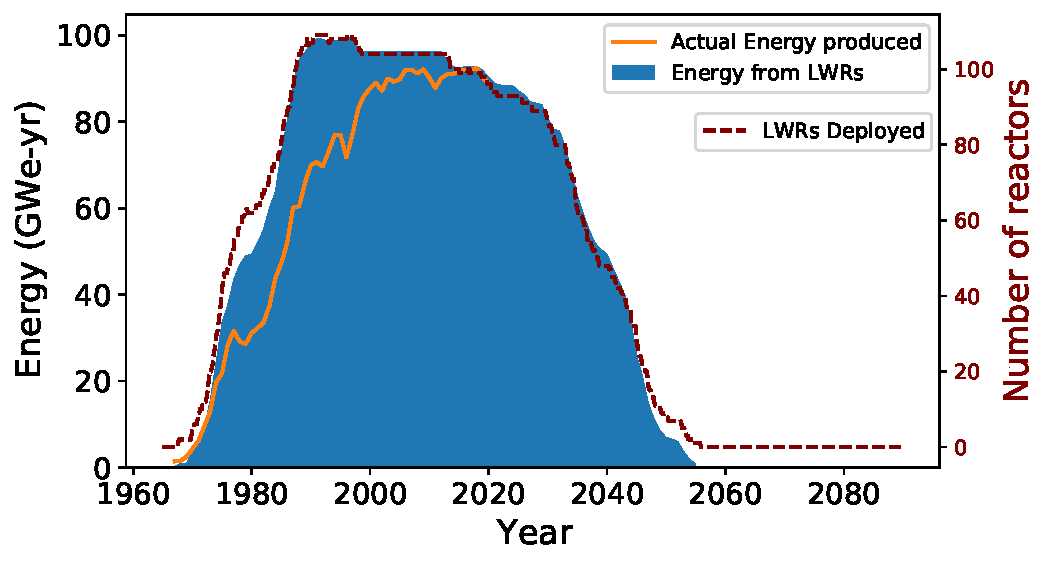
\includegraphics[scale=0.8]{s1_energy_reactors.pdf}
    \caption{Energy supplied by \glspl{LWR} in Scenario 1 during each year of
    the simulation compared to the number of reactors deployed.}
    \label{fig:energy_reactor1}
\end{figure}


The mass of enriched uranium sent to the \glspl{LWR} in this scenario (Figure 
\ref{fig:fuel1}) follows the general pattern of the reactor deployment, but with 
more variation between individual time steps. The increased variation between 
time steps is because of the staggering of outages for the reactors, or when 
they receive fuel. There are also times with large increases in the mass of fuel 
sent to the reactors, such as in 2016, because these times include the deployment 
of a new reactor with a full core of fuel instead of the amount that is 
sent for refueling. 

The maximum amount of enriched uranium sent to the \glspl{LWR} at any one 
time in this scenario is 513.72 MTU. The average mass of enriched uranium sent to 
the reactors for the entire scenario is 135.74 MTU/month. The average mass of 
enriched uranium sent to the \glspl{LWR} between when they are first deployed 
and 2025 is 164.92 MTU/month. This average is larger than what is reported in 
\cite{bachmann_enrichment_2021} because the average reported by 
Bachmann et. al accounts for the time before the \glspl{LWR} are actually 
deployed while the average reported here does not. The average mass of 
uranium sent to \glspl{LWR} between 2025-2055, from the start of the transition 
to when they are all decommissioned is 81.11 MTU/month. Comparing the averages 
shows that the vast majority of enriched uranium is sent to the \glspl{LWR} 
before 2025, which matches with the decline in the number of \glspl{LWR} 
deployed after 2020. After 2025, a cumulative total of 29,848.6 MTU is 
sent to the \glspl{LWR},
which is less than the cumulative mass reported in \cite{bachmann_enrichment_2021}
because Bachmann et al. assumed that all \glspl{LWR} would operate for 60 years, 
which is longer than the assumed operating time for some \glspl{LWR} in 
this work. This scenraio requires a total of 143,479 MT of enriched uranium.

\begin{figure}
    \centering
    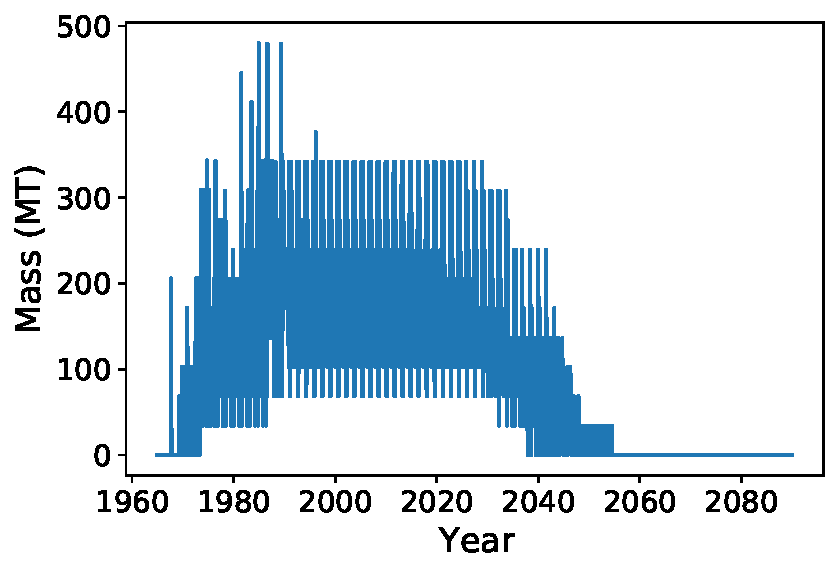
\includegraphics[scale=0.8]{s1_uox.pdf}
    \caption{Mass of uranium supplied to the LWRs in Scenario 1 at each time step.}
    \label{fig:fuel1}
\end{figure}

The next metric of interest for this work is the mass of natural uranium 
required as feed material to produce the enriched uranium for the 
reactors. The mass of feed uranium 
is about an order of magnitude larger than the mass of the enriched uranium 
(Figure \ref{fig:feed1}). Scenario 1 requires a maximum of 4,121.8 MT of 
feed uranium at one time and an average of 1,089.1 MT/month of natural uranium 
when \glspl{LWR} are deployed. Before 2025, this scenario requires an average of 
1,323.2 MTU/month of natural uranium, and requires an average of 650.8 MTU/month 
after 2025. In total, the \glspl{LWR} require 1,151,208 MT of feed uranium.

\begin{figure}
    \centering
    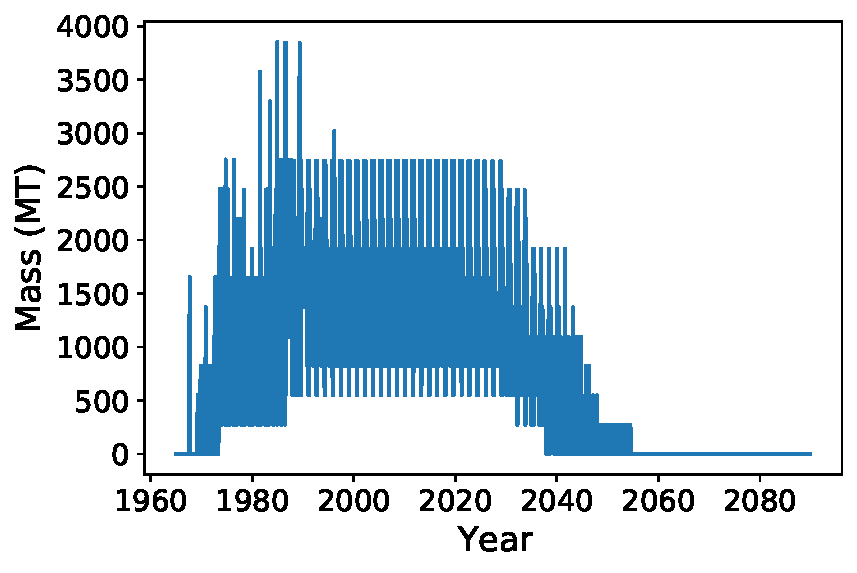
\includegraphics[scale=0.8]{s1_feed.pdf}
    \caption{Mass of natural uranium required to produce fuel for the LWRs at each 
    time step in Scenario 1.}
    \label{fig:feed1}
\end{figure}

The next metric of interest for this work is the \gls{SWU} capacity required 
to produce the enriched uranium for the \glspl{LWR}, 
shown in Figure \ref{fig:swu1}. This scenario requires a maximum of 3,714 MT-SWU 
to 
enrich the uranium sent to the reactors at one time step and an average of 
981.4 MT-SWU/month to enrich all of the uranium sent to 
the \glspl{LWR} when they are deployed. An average of 
1192.4 MT-SWU/month is required to produce the enriched uranium 
for \glspl{LWR} between their initial deployment and 2025, and 
586.4 MT-SWU/month is needed to produce the 
enriched uranium sent to \glspl{LWR} between 2025 and 2055. The values 
reported here are different than what Bachmann et al. \cite{bachmann_enrichment_2021}
reports for a few different reasons. The first reason is that these results  
consider only
the time steps in which the \glspl{LWR} are deployed while Bachmann et al. 
considers all time steps, similar to what leads to the differences in the 
reported mass of 
enriched uranium. The other reason
is the use of different enrichment levels for the \gls{LWR} fuel. 
Bachmann et al. assumes an enrichment of 4.5\% while this work assumes 4.3\%
$^{235}$U enrichment for \gls{LWR} fuel. 


\begin{figure}
    \centering
    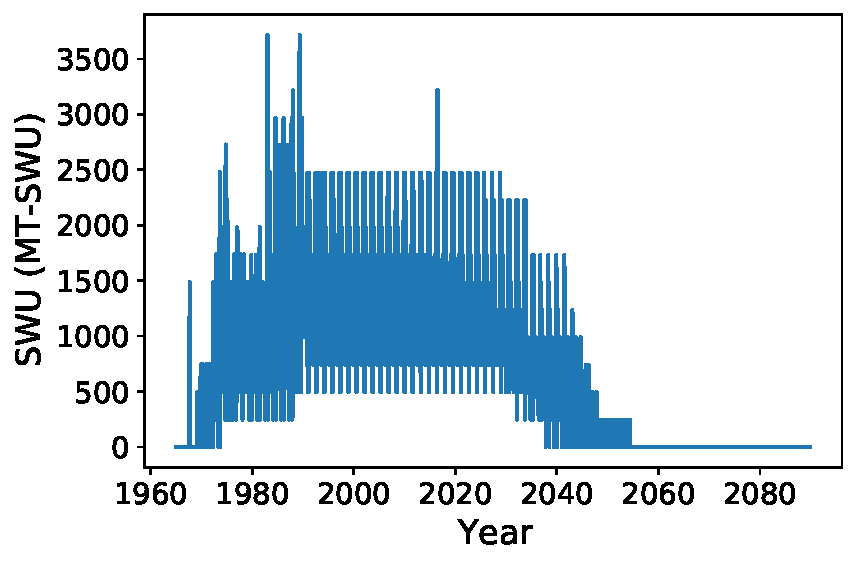
\includegraphics[scale=0.8]{s1_swu.pdf}
    \caption{SWU capacity required to enrich the uranium sent to LWRs at each time step in Scenario 1.}
    \label{fig:swu1}
\end{figure}

The last metric is the \gls{SNF} discharged from the reactors as a function of
time (Figure \ref{fig:waste1}). The \glspl{LWR} discharge a maximum of 393.6 MT 
of spent fuel in one time step and an average of 130.1 MT/month when they are 
deployed. Between the first \gls{LWR} deployment and 2025 the \glspl{LWR} 
dicharge an average of 149.5 MTU/month, and an average of 93.9 MT/month  
between 2025-2055. The \glspl{LWR} discharge a total of 137,581 MT of \gls{SNF} 
in Scenario 1. 

\begin{figure}
    \centering
    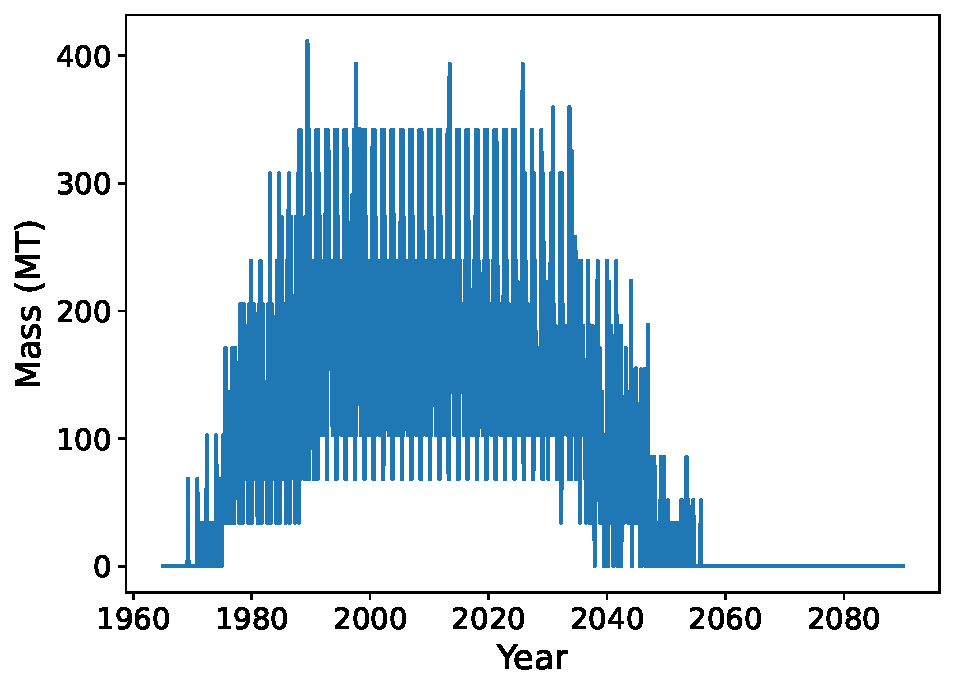
\includegraphics[scale=0.8]{s1_waste.pdf}
    \caption{Mass of spent fuel discharged from the reactors in Scenario 1 as a function of time.}
    \label{fig:waste1}
\end{figure}

\section{Energy Supplied}
\subsection{No growth scenarios}
The energy demand in the no growth scenarios (Scenarios 2-7) is a constant
89.456 GWe-yr, based on the energy supplied by the reactors in Scenario 1
in 2025. The energy supplied in Scenarios 2-7 does not fully meet the demand
throughout the duration of the transition (Figure \ref{fig:nogrowth_energy}). 
All of the 
transition scenarios experience the same energy production until 2030,
reaching a low point of 83.94 GWe-yr. Each of the scenarios exhibit variation 
in the annual energy production, which is a result of refueling 
periods for the \glspl{LWR} and any VOYGRs present. The maximum gap between 
energy production and demand is 5.516 GWe-yr, in Scenarios 4 and 7 
(Table \ref{tab:nogrowth_energy}). There 
is very little oversupply of energy in any of these scenarios, with a 
maximum oversupply of 0.018 GWe-yr in Scenario 3.

Throughout 
most of the time with advanced reactors, Scenario 6 generally has the 
lowest energy 
production, producing between 83.95-87.38 GWe-yr. Scenario 3 is able 
to best meet the demand, producing a constant 89.52 GWe-yr starting in 2056,
because the scenario only deploys the Xe-100, which has the longest lifetime 
and utilizes online refueling. These characteristics mean that the reactors 
are not being frequently replaced and do not have outages for refueling 
that decrease the energy produced in the simulation. Scenario 4 meets the 
energy demand the next best, producing at least 89.43 GWe-yr starting in 
2056, because this scenario primarily deploys Xe-100s. However, this scenario 
also deploys VOYGRs, which experiences a month-long refueling period 
every 18 months. This refueiling period contributes to the slightly lower 
energy produced in this scenario compared with Scenario 4 and the 
variation in the energy produced between years.
Because each scenario experiences times of not fully meeting the energy 
demand, one can assume that the material requirements reported for each 
scenario are an underestimate and that ensuring no times of 
energy undersupply would need additional reactors and materials.

\begin{figure}
    \centering
    \begin{subfigure}[b]{0.45\textwidth}
        \centering
        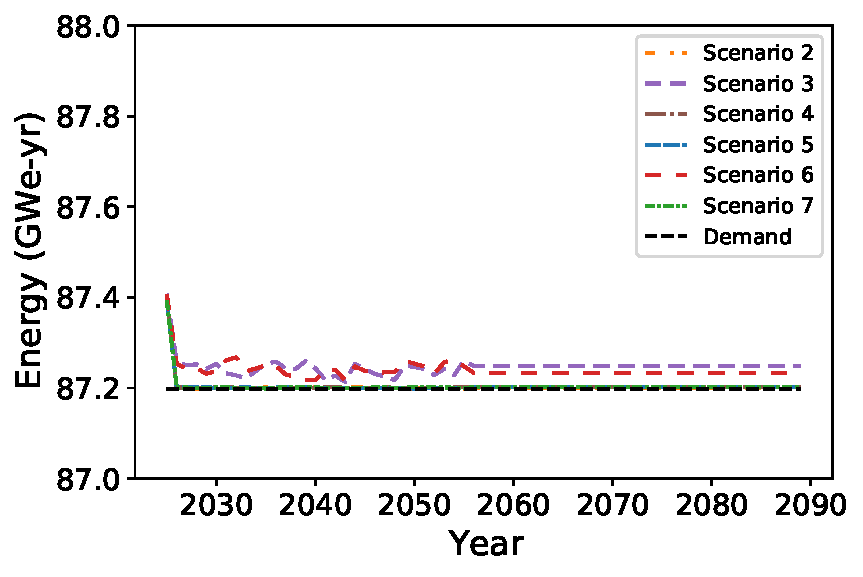
\includegraphics[width=\textwidth]{nogrowth_energy_after_2025.pdf}
        \caption{Annual energy produced compared to demand for Scenarios 2-7
        between 2025-2090.}
        \label{fig:nogrowth_energy_after_2025}
    \end{subfigure}
    \hfill
    \begin{subfigure}[b]{0.45\textwidth}
        \centering
        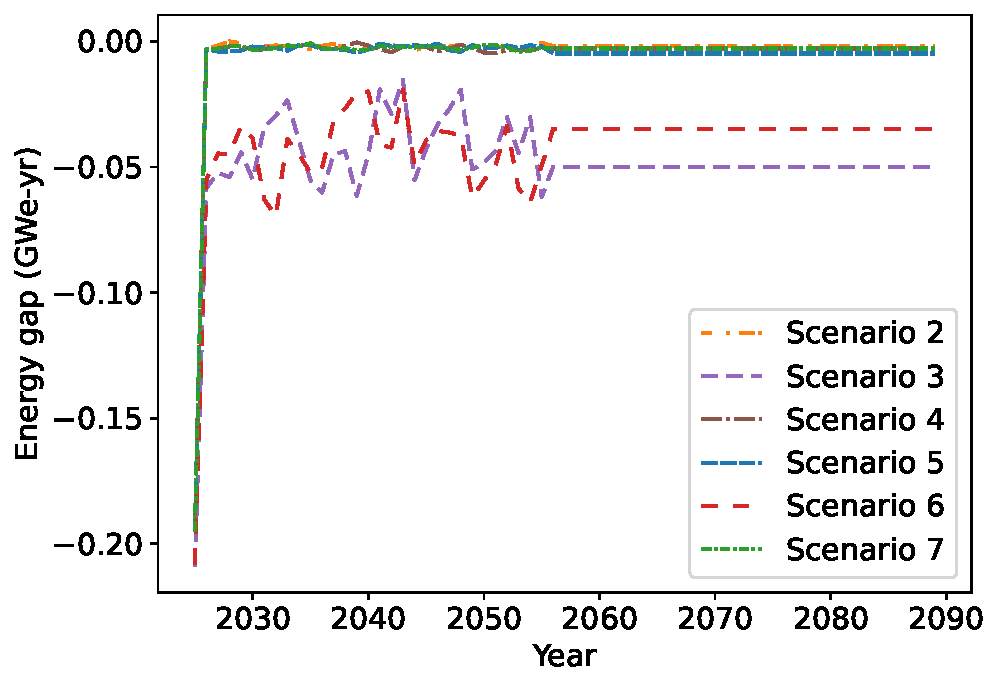
\includegraphics[width=\textwidth]{nogrowth_energy_gap.pdf}
        \caption{Gap between energy demand and energy produced by reactors 
        in Scenarios 2-7 between 2025-2090. Positive values indicate an 
        undersupply of energy and negative values represent an 
        oversupply of energy.}
        \label{fig:nogrowth_energy_gap}
    \end{subfigure}
       \caption{Annual energy produced comapred to demand in Scenarios 2-7.}
       \label{fig:nogrowth_energy}
\end{figure}

\begin{table}
    \centering
    \caption{Maximum undersupply and oversupply of energy in Scenarios 2-7.}
    \label{tab:nogrowth_energy}
    \begin{tabular}{c c c}
        \hline 
        Scenario & Max Oversupply (GWe-yr) & Max Undersupply (GWe-yr) \\
        \hline 
        2 & 0.003 & 5.516 \\
        3 & 0.063 & 5.468 \\
        4 & 0.003 & 5.516 \\
        5 & 0.000 & 5.516 \\
        6 & 0.000 & 5.502 \\
        7 & 0.000 & 5.516 \\
        \hline
        
    \end{tabular}
\end{table}

\subsection{1\% growth scenarios}
For the 1\% growth scenarios this is a similar gap between energy 
production and 
demand immediately after the transition start time. All of the 
scenarios have an energy deficit between 2025 and 2039. After 2039, Scenarios
8-10 provide an oversupply of energy. Scenario 12 begins to experience 
an oversupply of energy 2046, and Scenario 13 experiences an oversupply 
of energy beginning in 2042. Scenario 11 does not ever experience an 
oversupply of energy, and is at most just able to meet the demand at the 
beginning of the transition. 
The maximum gap between the energy demand 
and the energy supplied for any of the scenarios is 3.03 GWe-yr, experienced 
by Scenario 11 in 2033 (see Table \ref{tab:1percent_energy}). The 
initial gap in energy demand for each of these scenarios indicates that
this work underestimates the initial material requirements for the 
scenarios. However, the 
oversupply of energy for the later time steps for most of the scenarios 
indicates that the material requirements for these time steps will be 
accurate for the needs of the scenario. Scenarios 5 and 11 experience the 
largest gap between energy supply and demand, and both of these scenarios 
deploy the VOYGR and \gls{MMR}, indicating that this combination of 
reactors may not be ideal for using advanced reactors to meet energy 
demands. 

\begin{figure}
    \centering
    \begin{subfigure}[b]{0.45\textwidth}
        \centering
        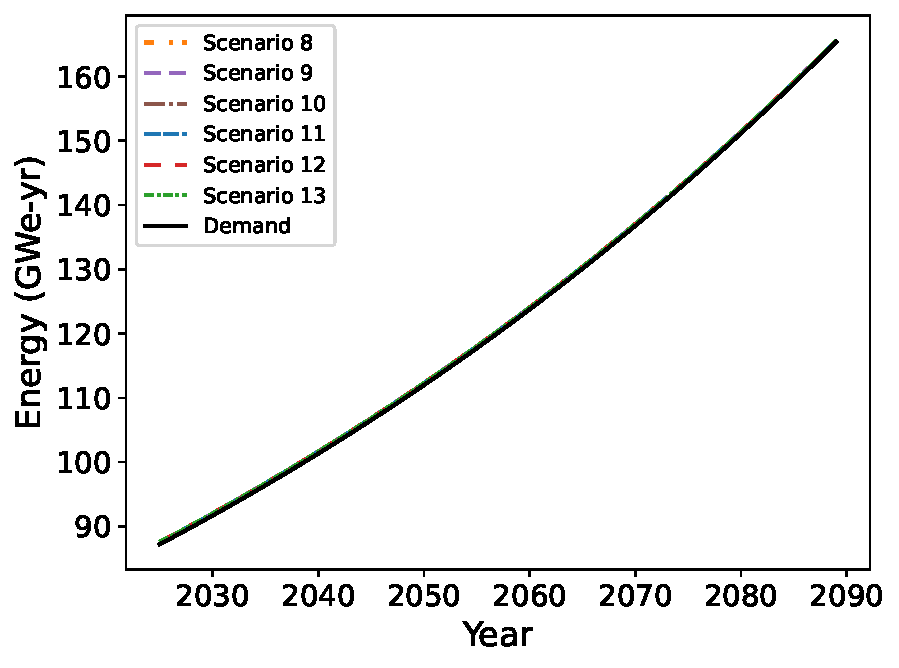
\includegraphics[width=\textwidth]{1percent_energy_after_2025.pdf}
        \caption{Annual energy produced compared to demand for Scenarios 8-13
        between 2025-2090.}
        \label{fig:1percent_energy_after_2025}
    \end{subfigure}
    \hfill
    \begin{subfigure}[b]{0.45\textwidth}
        \centering
        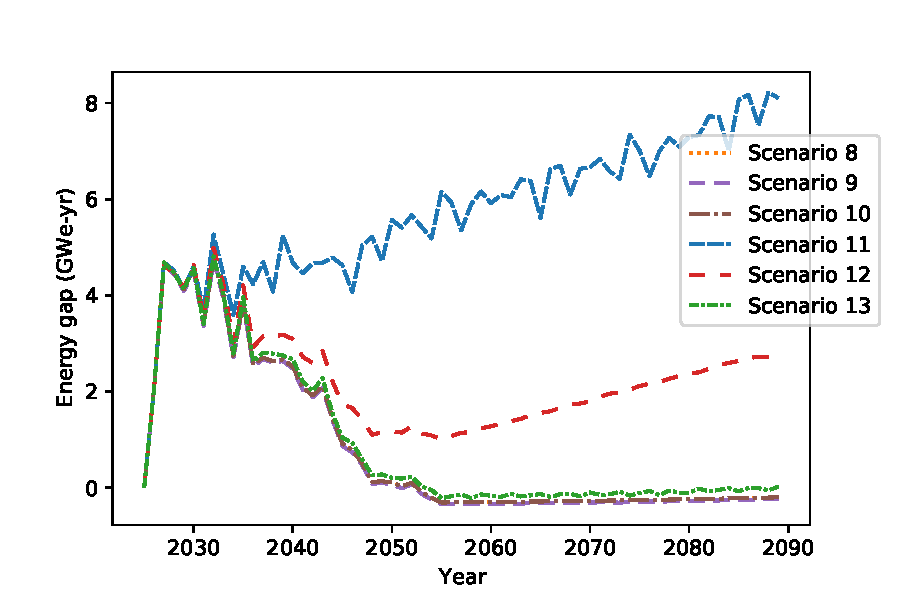
\includegraphics[width=\textwidth]{1percent_energy_gap.pdf}
        \caption{Gap between energy demand and energy produced in Scenarios 8-13
        between 2025-2090. Positive values represents an undersupply of energy 
        and negative values represents an oversupply of energy. }
        \label{fig:1percent_energy_gap}
    \end{subfigure}
       \caption{Annual energy produced compared to demand in Scenarios 8-13.}
       \label{fig:1percent_energy}
\end{figure}

\begin{table}
    \centering
    \caption{Maximum undersupply and oversupply of energy in Scenarios 8-13.}
    \label{tab:1percent_energy}
    \begin{tabular}{c c c}
        \hline 
        Scenario & Max Oversupply (GWe-yr) & Max Undersupply (GWe-yr) \\
        \hline 
        8 & 3.94 & 2.90 \\
        9 & 4.79 & 2.87 \\
        10 & 4.74 & 2.90 \\
        11 & 0.00 & 3.02 \\
        12 & 2.96 & 2.89 \\
        13 & 3.66 & 2.90\\
        \hline
        
    \end{tabular}
\end{table}

\section{Reactor deployment}
This section compares the scenarios on the number of advanced reactors 
built. This metric takes two 
different forms: the number of reactors that are in the simulation at 
one time, and the number of reactors that are built (enter the simulation)
in a single time step. These metrics combined provide insight into the 
number of reactors needed and the rate at which to build them. 

The \Cycamore \texttt{ManagerInst} institution archetype preferentially
deploys prototypes based on 
the order in which they are listed in the input file. The 
\texttt{ManagerInst} deploys the first prototype 
until deploying more would create a surplus of the required 
commodity (in this case power), then it deploys the next prototype 
until its deployment would create a surplus of the requried commodity, 
and so forth. 
Because of this scheme, the prototypes were listed in decreasing order of 
power 
output (i.e. Xe-100, VOYGR, then \gls{MMR}, for the necessary prototypes 
in that scenario). This scheme optimizes the scenario for the minimum 
number of reactors deployed and minimized oversupply of power. 
This ordering most closely 
matches a potentially implemented decision making process. 

\subsection{No growth scenarios}
Advanced reactors are first deployed in February 2030 for all scenarios, about 
5 years after transition start time. The delay between the start of the 
transition and the deployment of advanced reactors causes the deficit between 
energy demand and the energy produced in the transition scenarios. 
This initial deployment time is 
19 months earlier than the initial deployment time reported in 
\cite{bachmann_enrichment_2021}. The initial deployment time for advanced 
reactors for no growth transitions is only one month later than the 
initial deployment time reported in \cite{bachmann_enrichment_2021}
for 1\% growth transitions. 

The number of reactors deployed varies based on 
the type of reactor used in the scenario and scales with the power output of 
each type of reactor, as shown in Figure \ref{fig:nogrowth_reactors}. Scenario
2 requires the most reactors, because the \gls{MMR} has the smallest power 
output of the reactors considered in this work. Additionally, 17,892
\gls{MMR} are deployed 
at one time in Scenario 2 (Table \ref{tab:reactors_nogrowth}) to meet the 
power demand. Scenario 3 requires the smallest number of advanced reactors 
(1119) because this scenario only deploys the Xe-100, which
has the largest power output. 

\begin{figure}
    \centering
    \begin{subfigure}[b]{0.45\textwidth}
        \centering
        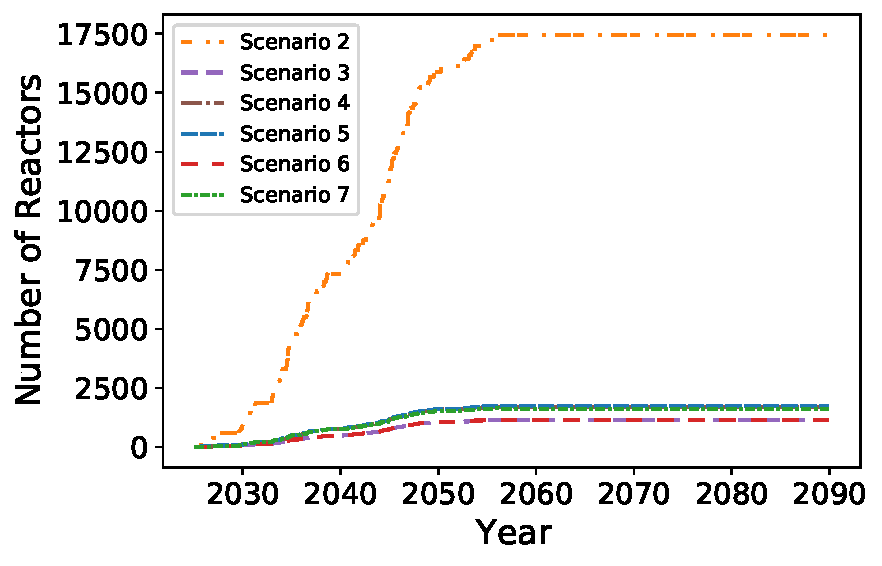
\includegraphics[width=\textwidth]{nogrowth_reactors.pdf}
        \caption{Total number of advanced reactors deployed at 
        each time step in Scenarios 2-7 between 2025-2090.}
        \label{fig:nogrowth_reactors_all}
    \end{subfigure}
    \hfill
    \begin{subfigure}[b]{0.45\textwidth}
        \centering
        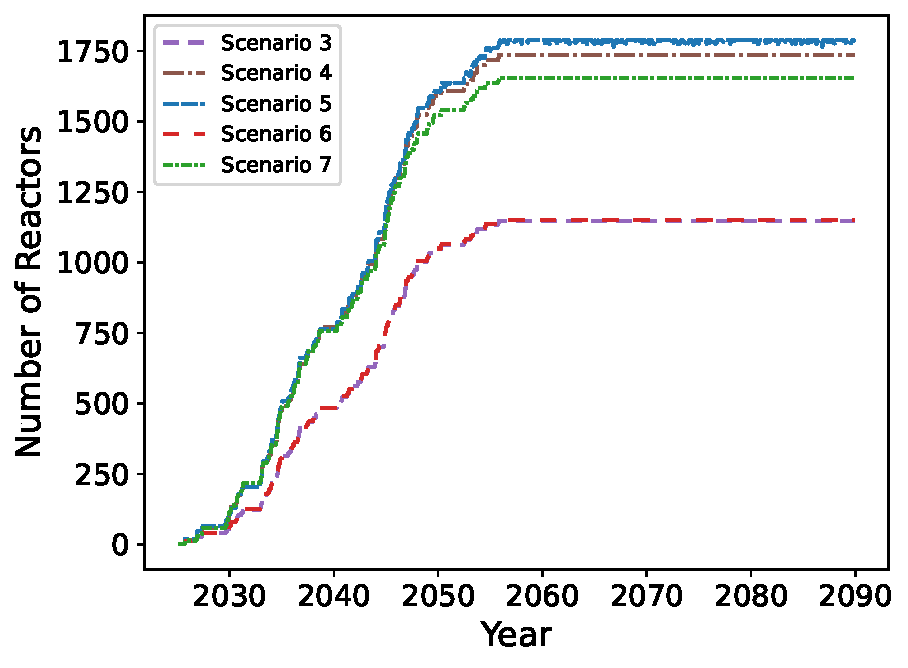
\includegraphics[width=\textwidth]{nogrowth_reactors_3-7.pdf}
        \caption{Total number of advanced reactors deployed at 
        each time step in Scenario 3-7 between 2025-2090.}
        \label{fig:nogrowth_reactors_3-7}
    \end{subfigure}
       \caption{Number of advanced reactors deployed at each time step 
       for Scenarios 2-7. The figures begin at 2025, because no advanced 
       reactors are deployed before then. In the right figure Scenario 
       2 is removed to highlight the trends in the other scenarios.}
       \label{fig:nogrowth_reactors}
\end{figure}

\begin{table}
    \centering 
    \caption{Maximum number of reactors deployed at one time in 
    Scenarios 2-7.}
    \label{tab:reactors_nogrowth}
    \begin{tabular}{c c c c c}
        \hline
        Scenario & \glspl{MMR} [\#] & Xe-100s [\#] & VOYGRs [\#] 
        & Total [\#]\\\hline
        2 & 17892 & - & - & 17892\\
        3 & - & 1119 & - & 1119\\
        4 & 475 & 1089 & - & 1557\\
        5 & 13361 & - & 766 & 13617\\
        6 & - & 328 & 821 & 1149\\
        7 & 5090 & 759 & 291 & 5832\\
        \hline
    \end{tabular}
\end{table}

Scenario 2 shows variation in the number of reactors deployed 
after 2050. The variation is a result of the shorter lifetime of the 
\gls{MMR} compared with the Xe-100 and VOYGR. The shorter lifetime 
means that the \glspl{MMR} must be decommissioned and commissioned more 
frequently than the other reactors. The variation observed in Scenario 2 
occurs on 20 year cycles.  
Scenarios 4 and 7, which also deploy the \gls{MMR}, exhibit similar 
variations, with a less pronounced variation 
than in Scenario 2 because fewer 
\glspl{MMR} are deployed in these scenarios.

Scenarios 5 and 7 show a decrease in the number of advanced 
reactors deployed with time. This decrease occurs because when the 
\glspl{MMR} retire they are replaced with either Xe-100s or VOYGRs 
instead of with more \glspl{MMR}. In Scenario 5 the \glspl{MMR} are 
replaced with VOYGRs and in Scenario 7 the \glspl{MMR} are mostly 
replaced with Xe-100s. The replacement of the \glspl{MMR} occurs 
because the gap between the power supplied and the demand becomes 
large enough to warrant the larger power output of the Xe-100 or VOYGR.
Scenarios 3 and 4 have a constant number of advanced reactors deployed 
starting in December 2055. These scenarios have a constant number of 
advanced reactors because by December 2055 all of the \glspl{LWR} have 
been decommissioned, so the only gap between energy supply and demand 
will come from the decommissioning of advanced reactors. The Xe-100 and 
the VOYGR have a 60 year lifetime, so any built after 2030 (which is all 
of them) will not be decommissioned on this time scale. 

In addition to the total number of each type of advanced reactor deployed 
at each time, the maximum number of each advanced reactor deployed in a 
single time step is reported (Table 
\ref{tab:reactors_added_nogrowth}). This information provides insight 
into the speed at which new reactors must be built. For scenarios with 
multiple advanced reactors, the numbers reported do not necessarily occur 
at the same time. Scenario 2 requires 
the largest number of reactors to be deployed at a single time, which 
is consistent with this scenario requiring a larger total number of 
reactors. Scenario 3 deploys the fewest reactors in 
a single time step, based on the total column of Table 
\ref{tab:reactors_added_nogrowth}, because of the larger power output from 
the Xe-100 compared with the other advanced reactors. 

\begin{table}
    \centering 
    \caption{Maximum number of reactors added to the simulation at a 
    single time step in Scenarios 2-7.}
    \label{tab:reactors_added_nogrowth}
    \begin{tabular}{c c c c c}
        \hline
        Scenario & \glspl{MMR} [\#]& Xe-100s [\#]& VOYGRs [\#]
        & Total[\#]\\\hline
        2 & 756 & - & - & 756\\
        3 & - & 47 & - & 47\\
        4 & 15 & 47 & - & 54\\
        5 & 679 & - & 5 & 684\\
        6 & - & 28 & 33 & 48\\
        7 & 430 & 41 & 20 & 436\\
        \hline
    \end{tabular}
\end{table}

\subsection{1\% growth scenarios}
All of the 1\% growth scenarios deploy advanced reactors beginning 
in September 2026, which is more 
than three years before their initial deployment for a 1\% growth 
transition as reported in \cite{bachmann_enrichment_2021} and 38 months 
earlier than in the no growth scenarios. Despite this earlier deployment, 
there is still the gap between the energy supplied and the demand 
(Figure \ref{fig:1percent_energy}). This suggests that to meet a 1\% 
growth in demand advanced reactors would need to be deployed even earlier, 
possibly even before 2025. 

The number of reactors deployed in these scenarios is similar to the 
trends observed for the no growth scenarios. Transitioning to only the 
\gls{MMR} (Scenario 8) requires the largest number of reactors, and 
transitioning to only the Xe-100 (Scenario 9) requires the fewest 
number of advanced reactors. Scenarios 10 and 13 have similar numbers of 
reactors deployed, as do Scenarios 9 and 12. 

Regarding the rate of reactor deployment, Scenario 8 deploys the most 
reactors in a single time step (Table 
\ref{tab:reactors_added_1percent}), with 412 \glspl{MMR} deployed at once. 
Scenario 11 requires the next largest number of reactors deployed in 
a single time step, 77 VOYGRs in one step and 79 total advanced reactors. 
The other scenarios all have comparable numbers, around 50 reactors 
deployed at once. Scenarios 9 and 12 require the same number of 
advanced reactors deployed in the same time step. 

\begin{figure}
    \centering
    \begin{subfigure}[b]{0.45\textwidth}
        \centering
        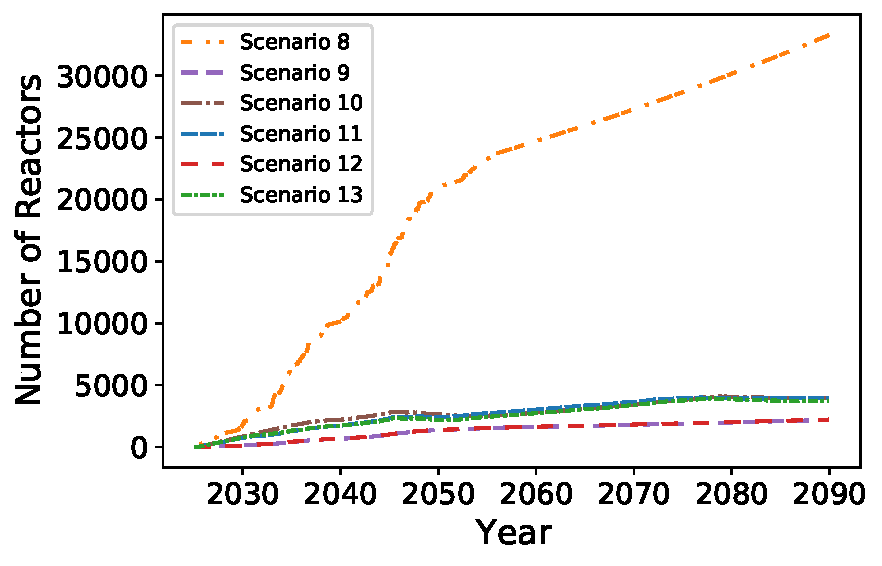
\includegraphics[width=\textwidth]{1percent_reactors.pdf}
        \caption{Total number of advanced reactors deployed at 
        each time step in Scenarios 8-13 between 2025-2090.}
        \label{fig:1percent_reactors_all}
    \end{subfigure}
    \hfill
    \begin{subfigure}[b]{0.45\textwidth}
        \centering
        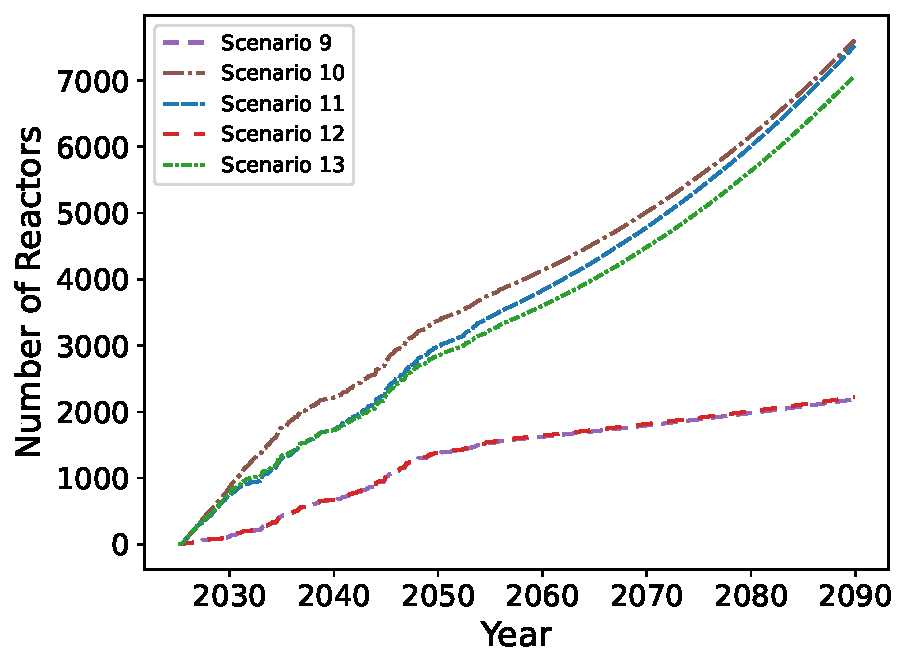
\includegraphics[width=\textwidth]{1percent_reactors_9-13.pdf}
        \caption{Total number of advanced reactors deployed at 
        each time step in Scenario 9-13 between 2025-2090.}
        \label{fig:1percent_reactors_9-13}
    \end{subfigure}
       \caption{Number of advanced reactors deployed at each time step 
       for Scenarios 8-13. The figures begin at 2025, because no advanced 
       reactors are deployed before then. In the right figure Scenario 
       8 is removed to help highlight the trends in the other scenarios.}
       \label{fig:1percent_reactors}
\end{figure}

\begin{table}
    \centering 
    \caption{Maximum number of ereactors deployed in Scenarios 8-13.}
    \label{tab:reactors_1percent}
    \begin{tabular}{c c c c c}
        \hline
        Scenario & \glspl{MMR} [\#]& Xe-100s [\#]& VOYGRs [\#] 
        & Total [\#]\\\hline
        8 & 17467 & - & - & 17467\\
        9 & - & 2335 & - & 2335 \\
        10 & 1671 & 2119 & - & 3743\\
        11 & 699 & - & 3408 & 3869\\
        12 & - & 1678 & 1736 & 2663\\
        13 & 1432 & 1737 & 622 & 3746\\
        \hline
    \end{tabular}
\end{table}

\begin{table}
    \centering 
    \caption{Maximum number of reactors deployed in a single time step for 
    Scenarios 8-13.}
    \label{tab:reactors_added_1percent}
    \begin{tabular}{c c c c c}
        \hline
        Scenario & \glspl{MMR} [\#] & Xe-100s [\#] & VOYGRs [\#] 
        & Total [\#]\\\hline
        8 & 412 & - & - & 412\\
        9 & - & 52 & - & 52\\
        10 & 49 & 50 & - & 62\\
        11 & 4 & - & 77 & 79\\
        12 & - & 51 & 4 & 52\\
        13 & 49 & 50 & 28 & 62\\
        \hline
    \end{tabular}
\end{table}

\section{Uranium resources}
This section of results considers  
both the mass of enriched uranium and the mass of natural uranium feed 
required at each time step by each scenario. The feed uranium masses 
considered are the masses needed at an enrichment facility,
and does not account for any process losses between mining and 
enrichment. Therefore, the values reported are not the same as what would 
need to be mined. The masses of uranium resources are divided into four 
different metrics: the average monthly mass of uranium to supply all 
advanced reactors, the average monthly mass of \gls{HALEU} to supply 
advanced reactors, the maximum mass of uranium required by all advanced 
reactors in a single time step, and the cumulative mass required by the 
scenario. Each of these metrics provide information 
on how to design facilities to meet average and peak demands for 
uranium. The monthly averages are calculated beginning in January 2025, 
when the transition begins, which is not when the advanced reactors 
are first deployed. Therefore, the reported averages are slightly lower 
than if they were calculated starting at the advanced reactor deployment 
time. 
This methodology to report this result provides an average for if 
facilities are built to support the front-end of the \gls{NFC} starting 
in January 2025. 

\subsection{No growth scenarios}
The mass of enriched uranium sent to reactors (Fig. \ref{fig:nogrowth_uranium})
varies based on the advanced reactors deployed in the scenario. 
Scenario 2 has the largest average mass of enriched uranium sent to 
reactors each month, followed by Scenario 5 (Table 
\ref{tab:nogrowth_uranium}). The larger averages for these scenarios are 
because Scenario 2 deploys a large number of reactors deployed and 
because Sceario 5 deploys mostly VOYGRs, which 
require the largest mass of uranium in the core.
Scenarios 2 and 5 also require the largest mass of enriched uranium sent 
to advanced reactors at one time, with Scenario 2 requiring the msot. 
Scenario 3 requires the smallest average 
mass of enriched uranium, because this scenario deploys the fewest number 
of reactors and it deploys only the Xe-100 which requires the smallest 
uranium mass per core loading. All of the scenarios require a smaller 
average mass of enriched uranium than the \glspl{LWR} before 2025. 

Scenarios 2 requires the largest average mass of \gls{HALEU}, because 
of the large number of \glspl{MMR} deployed in this scenario. Scenario 
6 requires the smallest average mass of \gls{HALEU}, despite requiring the 
largest average mass of enriched uranium because most of the 
reactors in Scenario 6 are VOYGRs, which do not require \gls{HALEU}. 
The deployment 
of VOYGRs in tandem with \glspl{MMR} (Scenario 5) also results in a 
decrease in the average 
mass of \gls{HALEU} required, but the decrease is smaller in magnitude. 

Scenarios 2 and 5 require the largest mass of enriched uranium at a single 
time step. For Scenario 2, the large difference between the average and 
maximum amount of uranium is because of the refueling scheme for the 
\gls{MMR}. The \gls{MMR} only requires fuel when it is first being 
commissioned, therefore they do not require uranium at time periods in 
which
new reactors are not deployed. In Scenario 5, 958.5 MTU (99.6\%) of the 
maximum enriched uranium 
mass is non-\gls{HALEU} for the VOYGRs. The large difference between the 
monthly average and the maximum presents challenges in designing facilities 
to meet the demand. Designing such a facility would have to consider the 
material demands while also limiting the amount of stockpiled enriched 
uranium at the facility, because this is considered a proliferation risk. 

Finally, Scenario 6 requires the largest cumulative mass of enriched uranium 
for the no growth scenarios, which is consistent with Scenario 6 requiring 
the largest average monthly mass of enriched uranium.  Scenario 3 requires the 
smallest cumulative 
mass of enriched uranium, which is consistent with this scenario requiring 
the smallest average mass. The advanced reactors 
in all of these scenarios require a smaller cumulative mass of fuel than 
the \glspl{LWR}. Additionally, deploying the VOYGR in tandem with the other 
advanced reactors results in an increase in the cumulative mass 
of enriched uranium needed (e.g., Scenario 3 compared with Scenario 6). This
trend suggests that deploying VOYGRs increases the enriched uranium needs 
of the fuel cycle, even if it decreases the amount of \gls{HALEU} needed. 

\begin{figure}
    \centering
    \begin{subfigure}[b]{0.45\textwidth}
        \centering
        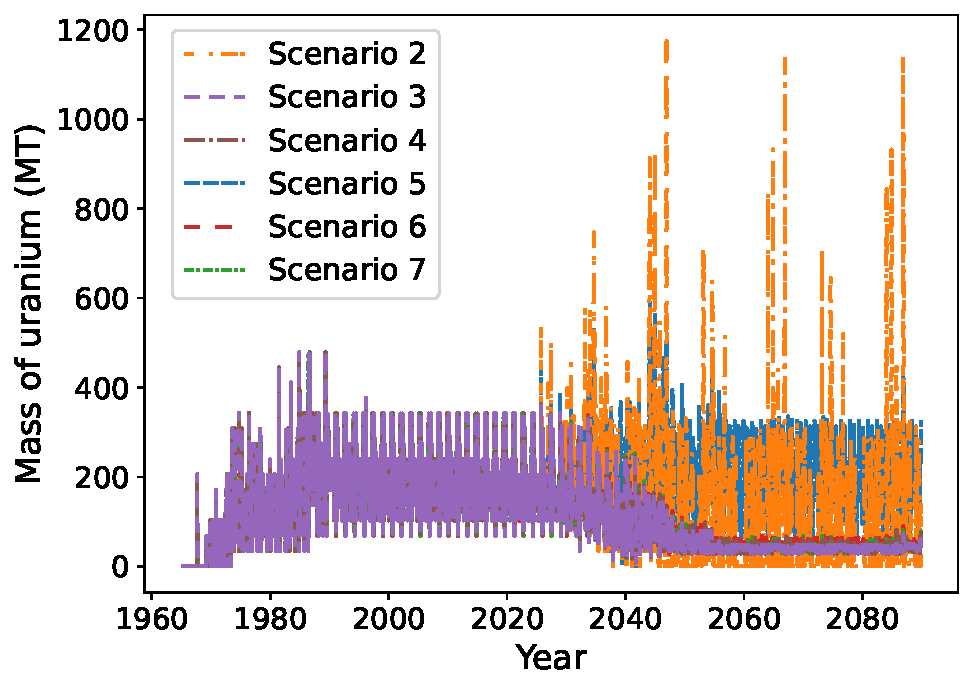
\includegraphics[width=\textwidth]{nogrowth_uranium.pdf}
        \caption{Mass of enriched uranium sent to all reactors 
        between 1965-2090.}
        \label{fig:nogrowth_all_uranium}
    \end{subfigure}
    \hfill
    \begin{subfigure}[b]{0.45\textwidth}
        \centering
        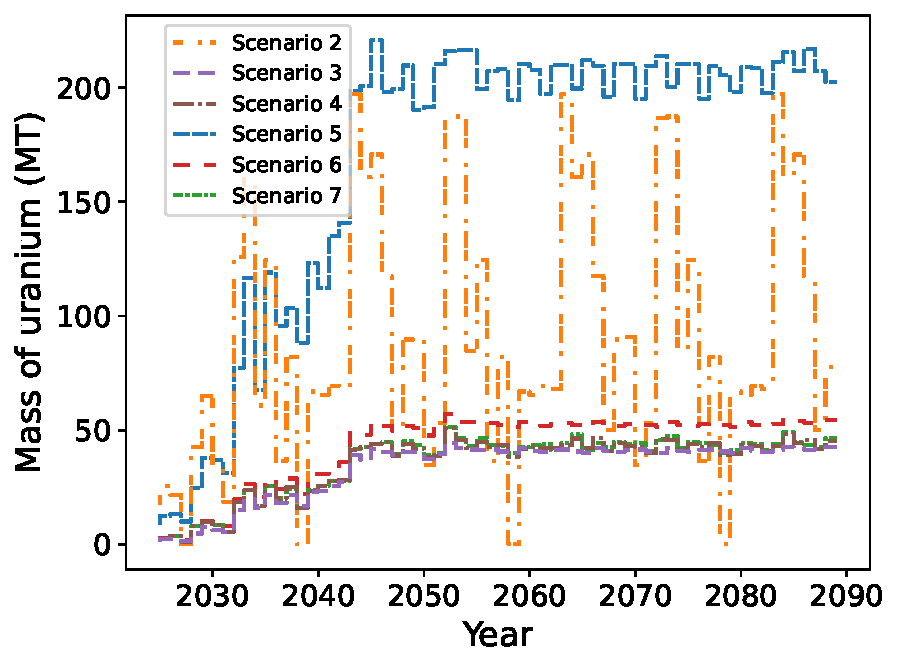
\includegraphics[width=\textwidth]{nogrowth_AR_uranium.pdf}
        \caption{Mass of enriched uranium sent to advanced reactors 
        between 2025-2090.}
        \label{fig:nogrowth_AR_uranium}
    \end{subfigure}
    \begin{subfigure}[b]{0.45\textwidth}
        \centering
        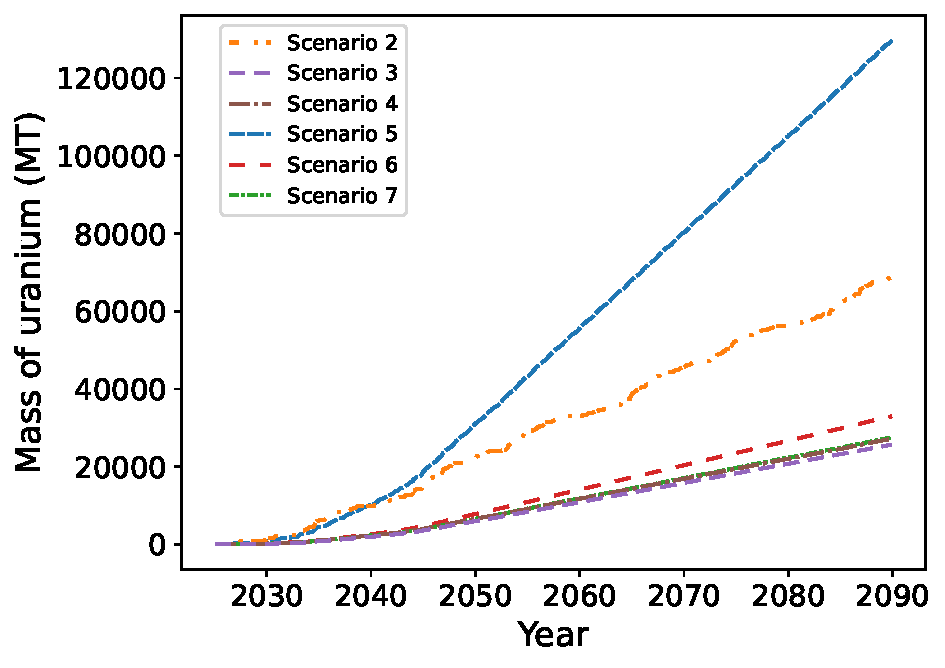
\includegraphics[width=\textwidth]{nogrowth_uranium_cumulative.pdf}
        \caption{Cumulative mass of enriched 
        uranium sent to advanced reactors between 2025-2090.}
        \label{fig:nogrowth_uranium_cumulative}
    \end{subfigure}
       \caption{Total mass of enriched uranium required by reactors
       at each time step in Scenarios 2-7.}
       \label{fig:nogrowth_uranium}
\end{figure}

\begin{table}
    \centering 
    \caption{Metrics for enriched uranium sent to advanced 
    reactors between 2025-2090 in Scenarios 2-7.}
    \label{tab:nogrowth_uranium}
    \begin{tabular}{c c c c c}
        \hline
        Scenario & Average (MT/month) & \gls{HALEU} Average 
        (MT/month) & Maximum (MT)& Cumulative (MT)\\\hline
        2 & 88.51 & 88.51 & 1,007 & 68,948\\
        3 & 31.53 & 31.53 & 86.79 & 24,562\\
        4 & 32.99 & 32.99 & 101.9 & 25,700\\
        5 & 117.8 & 48.99 & 1,015 & 91,760\\
        6 & 124.4 & 9.233 & 524.2 & 96,894\\
        7 & 73.06 & 31.89 & 652.6 & 56,914\\
        \hline
    \end{tabular}
\end{table}


For the mass of feed uranium, Scenario 2 requires the largest average mass 
to supply the advanced reactors (Figure \ref{fig:nogrowth_feed}, Table 
\ref{tab:nogrowth_feed}). Scenario 5 requires the next largest average 
mass of feed uranium, and requires less feed uranium than Scenario 2 because 
most of the product uranium for this scenario is for the VOYGRs, which 
require a lower enrichment assay than the \glspl{MMR}. Based on Eq. 
\ref{eq:enrichment_assasys}, a lower assay of the product stream results in 
a lower mass of feed material required. Scenario 5 still requires more feed 
material than the other scenarios because the average product mass required 
is much larger than the other scenarios, which offsets some of the decrease 
in feed material from the decrease in the product assay. 

\begin{figure}
    \centering
    \begin{subfigure}[b]{0.45\textwidth}
        \centering
        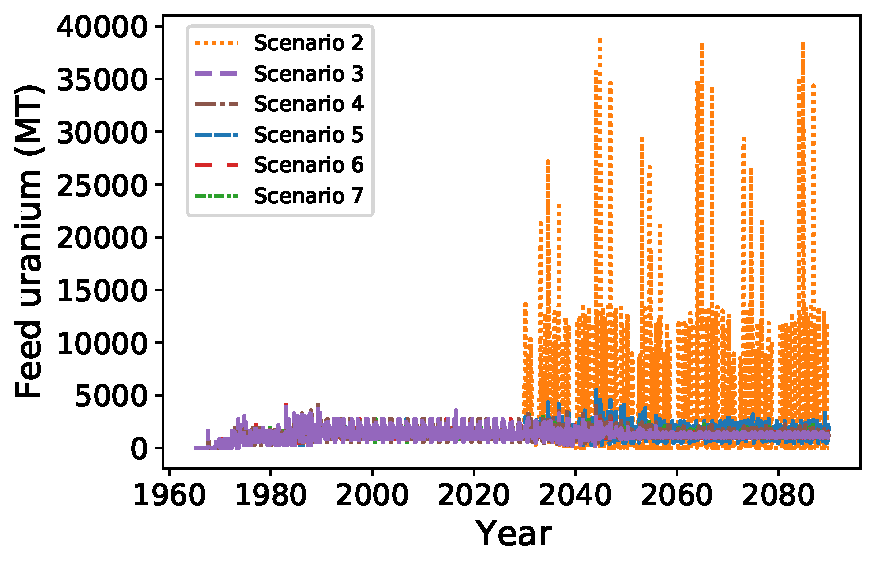
\includegraphics[width=\textwidth]{nogrowth_feed.pdf}
        \caption{Mass of feed uranium to produce enriched uranium sent to 
        all reactors between 1965-2090.}
        \label{fig:nogrowth_all_feed}
    \end{subfigure}
    \hfill
    \begin{subfigure}[b]{0.45\textwidth}
        \centering
        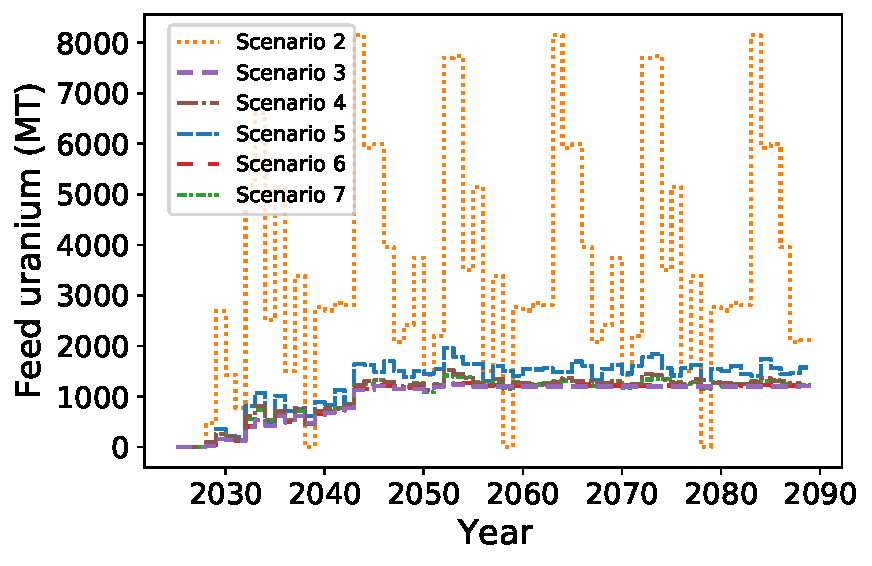
\includegraphics[width=\textwidth]{nogrowth_AR_feed.pdf}
        \caption{Mass of feed uranium to produce enriched uranium sent to 
        advanced reactors between 2025-2090.}
        \label{fig:nogrowth_AR_feed}
    \end{subfigure}
    \begin{subfigure}[b]{0.45\textwidth}
        \centering
        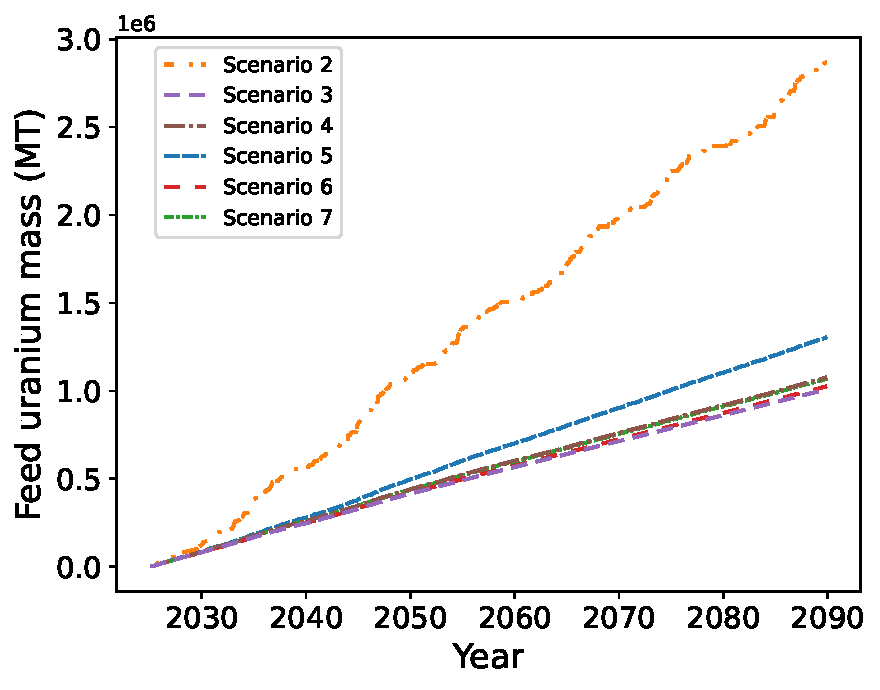
\includegraphics[width=\textwidth]{nogrowth_feed_cumulative.pdf}
        \caption{Cumulative mass of feed uranium to produce enriched 
        uranium for advanced reactors between 2025-2090.}
        \label{fig:nogrowth_feed_cumulative}
    \end{subfigure}
       \caption{Mass of feed uranium required to produce enriched uranium
        in Scenarios 2-7.}
       \label{fig:nogrowth_feed}
\end{figure}

\begin{table}
    \centering 
    \caption{Metrics for feed uranium required by advanced reactors 
    between 2025-2090 in Scenarios 2-7.}
    \label{tab:nogrowth_feed}
    \begin{tabular}{c c c c c}
        \hline
        Scenario & Average (t/month) & \gls{HALEU} Average 
        (t/month) & Maximum (t) & Cumulative (t)\\\hline
        2 & 3,386 & 3,386 & 38,517 & 2,637,870\\
        3 & 944.1 & 944.1 & 2,598 & 735,429\\
        4 & 1,007 & 1,007 & 3,184 & 784,536\\
        5 & 2,389 & 1,874 & 35,440 & 1,868,074\\
        6 & 1,153 & 276.4 & 4,909 & 898,210\\
        7 & 1,381 & 1,068 & 22,583 & 1,076,127\\
        \hline
    \end{tabular}
\end{table}

When comparing the feed material to create \gls{HALEU} in each scenario, 
Scenarios 2 and 5 require the most feed material. Scenario 6 
requires the least feed material to produce \gls{HALEU} because the vast 
majority of 
the reactors in this scenario are VOYGRs that do not require \gls{HALEU}.
Additionally, fueling the Xe-100 requires less feed uranium than fueling 
the \gls{MMR} because the Xe-100 requires a lower product assay and a 
smaller product mass per core. 
Scenarios 3, 4, and 7 require similar feed uranium masses (about 1,000 MTU/month)
despite Scenario 7 deploying a few hundred reactors more than the 
other scenarios. 
Scenario 7 deploys \glspl{MMR} in addition to the Xe-100s and VOYGRs,
which leads to the additional reactors in Scenario 7 and the decrease in 
the average feed material required because of the periods of no fuel being 
sent to the \glspl{MMR}. Deploying VOYGRs alongside the other advanced 
reactors (e.g., between Scenarios 3 and 6) generally decreases the average 
mass of feed uranium to create \gls{HALEU}, with the exception of deploying 
them alongside both \gls{HALEU}-fueled reactors (going from Scenario 4 to 
Scenario 7). Scenario 7 requiers a larger average mass of \gls{HALEU} than 
Scenario 4 because more \glspl{MMR} are deployed in Scenario 7. Therefore, 
Scenario 7 has more reactors that require \gls{HALEU}, increasing the 
demand for \gls{HALEU}.

The maximum feed uranium required by each scenario poses some 
challenge in facility design. The maximum feed uranium required varies 
between 2.7-14.8 times larger than the average feed material, which means 
that 
facilities to produce feed uranium will likely need to be designed with a 
larger capacity than the average feed uranium required to meet the peaks. 
The cumulative mass of feed uranium required by each scenario ranges between 
730,000-940,000 MTU for every scenario except Scenarios 2 and 5. 
Scenario 2 requires over 2.63 million MT and 
Scenario 5 requires almost 1.87 million MT of feed uranium, with the 
advanced reactors in both Scenarios 2 and 5 requiring more feed uranium 
than the \glspl{LWR}. The \gls{EIA} reports 
about 176,000 MT of U$_3$O$_8$ reserves in the US available at up to 
\$100/pound at the end of 2019 \cite{us_eia_2020_2021}, which is about 
149,000 MT of uranium. Therefore, the US must consider either uranium 
from international sources or uranium reserves at increased 
prices to meet the cumulative demand of feed 
uranium for each of these scenarios.

\subsection{1\% growth scenarios}
Most of the trends observed in the 1\% growth scenarios match the trends 
observed with the no growth scenarios that deploy the same reactor 
types
(Figure \ref{fig:1percent_uranium} and Table \ref{tab:1percent_uranium}). 
Scenario 11 requires the largest average mass of enriched uranium, but Scenario
12 requires the next largest average. This deviates from the no growth 
scenarios, in which Scenario 2 (\glspl{MMR} only) required the second largest 
average mass of enriched uranium. Scenario 12 requires the second largest 
average mass of enriched uranium because it deploys VOYGRs throughout 
the simulation to meet the energy demand, and the VOYGR requires the largest 
mass of uranium in the core. Therefore the enriched uranium demand increases 
more than if the same number of Xe-100s or \glspl{MMR} were deployed. 
This result shows how the assumed energy growth 
of the transitions impacts the scenario material requirements. 
Scenario 8 requires the largest average
mass of \gls{HALEU}, while Scenario 11 requires the least, and the other 
scenarios require less than 100 MT/month. This trend is consistent with 
the no growth scenarios. When comparing the average 
\gls{HALEU} mass required, the 1\% growth scenarios require almost twice 
the monthly average as the no growth scenarios. 

The maximum mass of enriched uranium required in each scenario ranges 
between 2.1-7.44 times the average monthly mass, which is a smaller increase 
than for the no growth scenarios. The increase between 
the average and the maximum is smaller for the 1\% growth scenarios because
the averages increase more than the maximums for the scenarios deploying the 
same reactors (e.g., between Scenarios 2 and 8). Scenario 9 requires the 
smallest monthly average of enriched uranium, because this scenario 
deploys the least number of reactors, and the Xe-100 requires the smallest 
mass of fuel in the core. The cumulative mass 
of enriched uranium required has a similar pattern to the average mass;
Scenario 11 requires the most mass, followed by Scenarios 12 
and 8. The advanced reactors in Scenario 11 require more enriched uranium 
than the \glspl{LWR}. 

\begin{figure}
    \centering
    \begin{subfigure}[b]{0.45\textwidth}
        \centering
        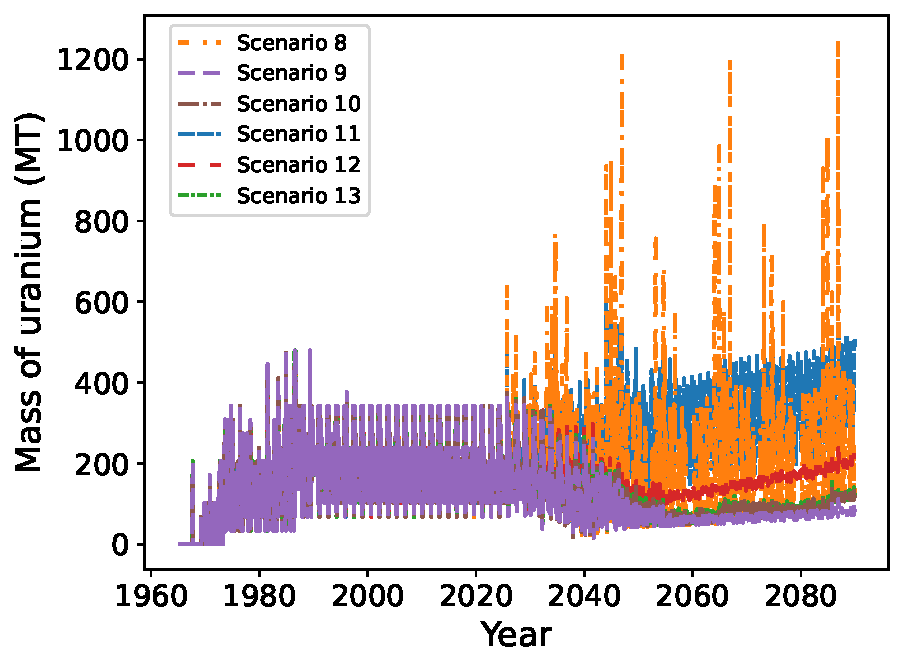
\includegraphics[width=\textwidth]{1percent_uranium.pdf}
        \caption{Mass of uranium sent to all reactors between 1965-2090.}
        \label{fig:1percent_all_uranium}
    \end{subfigure}
    \hfill
    \begin{subfigure}[b]{0.45\textwidth}
        \centering
        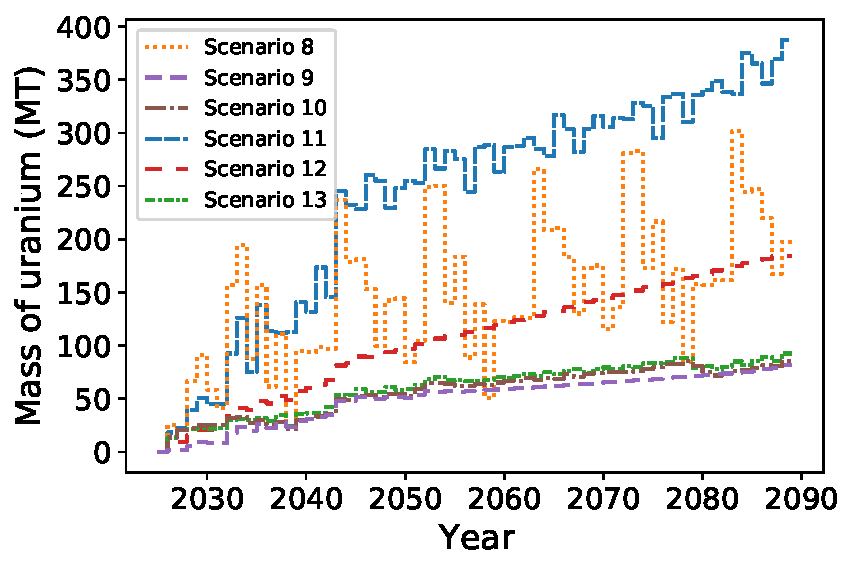
\includegraphics[width=\textwidth]{1percent_AR_uranium.pdf}
        \caption{Mass of enriched uranium sent to advanced reactors 
        between 2025-2090.}
        \label{fig:1percent_AR_uranium}
    \end{subfigure}
    \begin{subfigure}[b]{0.45\textwidth}
        \centering
        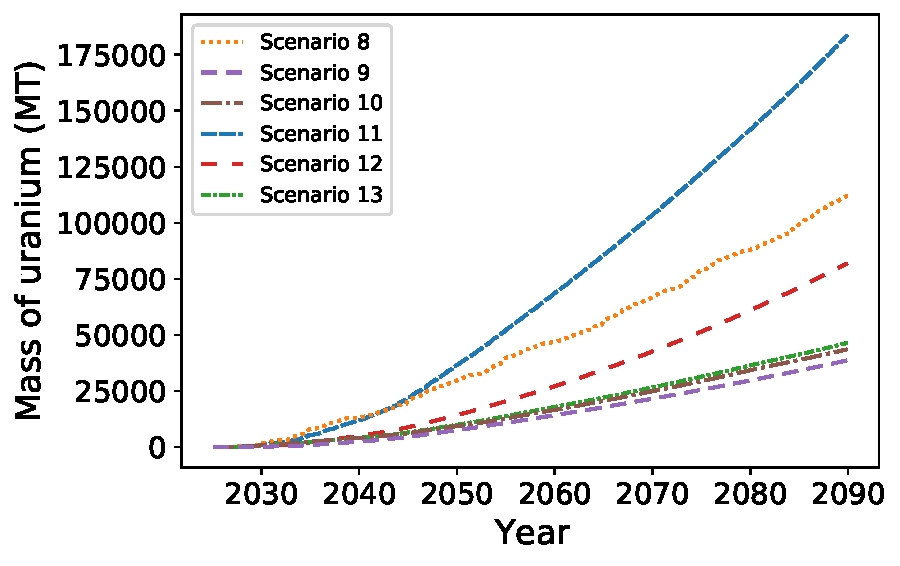
\includegraphics[width=\textwidth]{1percent_uranium_cumulative.pdf}
        \caption{Cumulative mass of enriched uranium sent to advanced reactors 
        between 2025-2090.}
        \label{fig:1percent_uranium_cumulative}
    \end{subfigure}
       \caption{Mass of enriched uranium required by reactors
        in Scenarios 8-13.}
       \label{fig:1percent_uranium}
\end{figure}

\begin{table}
    \centering 
    \caption{Metrics for enriched uranium required by advanced reactors 
    between 2025-2090 in Scenarios 8-13.}
    \label{tab:1percent_uranium}
    \begin{tabular}{c c c c c}
        \hline
        Scenario & Average (t/month) & \gls{HALEU} Average  
        (t/month) & Maximum (t) & Cumulative (t)\\\hline
        8 & 105.9 & 105.9 & 788.1 & 82,506\\
        9 & 56.99 & 56.99 & 118.4 & 44,398\\
        10 & 62.44 & 62.44 & 159.0 & 48,640\\
        11 & 254.4 & 4.142 & 1,018 & 198,165\\
        12 & 106.6 & 43.26 & 228.9 & 83,025\\
        13 & 95.69 & 52.05 & 357.8 & 74,542\\
        \hline
    \end{tabular}
\end{table}

The mass of feed uranium required by Scenarios 8-13 (Figure \ref{fig:1percent_feed},
Table \ref{tab:1percent_feed}) is similar with deviations in
Scenarios 8 and 11. Scenario 8 requires the 
most feed uranium based on any of the metrics in Table \ref{tab:1percent_feed},
because of the larger number of 
reactors deployed than the other scenarios and all of the reactors deployed 
require \gls{HALEU}. The larger product assay of \gls{HALEU}, compared with 
the product assay for \glspl{LWR} or VOYGRs, means that more 
feed uranium is needed to produce the same product mass (Eq. 
\ref{eq:enrichment_assasys}). Scenario 11 requires the next largest amount 
of 
feed uranium, with most of the feed uranium used to produce enriched 
uranium for the VOYGRs. The other scenarios require similar monthly 
averages of feed uranium, but there is some variation in how much of 
that feed uranium is used to produce \gls{HALEU}. 

The maximum feed uranium required varies between 2.1-7.4 times the monthly 
average of all feed uranium, which is similar to the 
mass of enriched uranium. Scenario 8 requires the largest maximum peak of 
feed uranium, corresponding to the deployment of many reactors. Because of 
the large number of reactors and the large mass of feed uranium required 
in Scenario 8, the cumulative mass of feed uranium quickly diverges from 
the cumualive mass of the other scenarios after the transition start time. 
Scenario 11 also deviates in the cumulative feed uranium 
mass required, but the deviation is not noticeable until around 
2045. 

\begin{figure}
    \centering
    \begin{subfigure}[b]{0.45\textwidth}
        \centering
        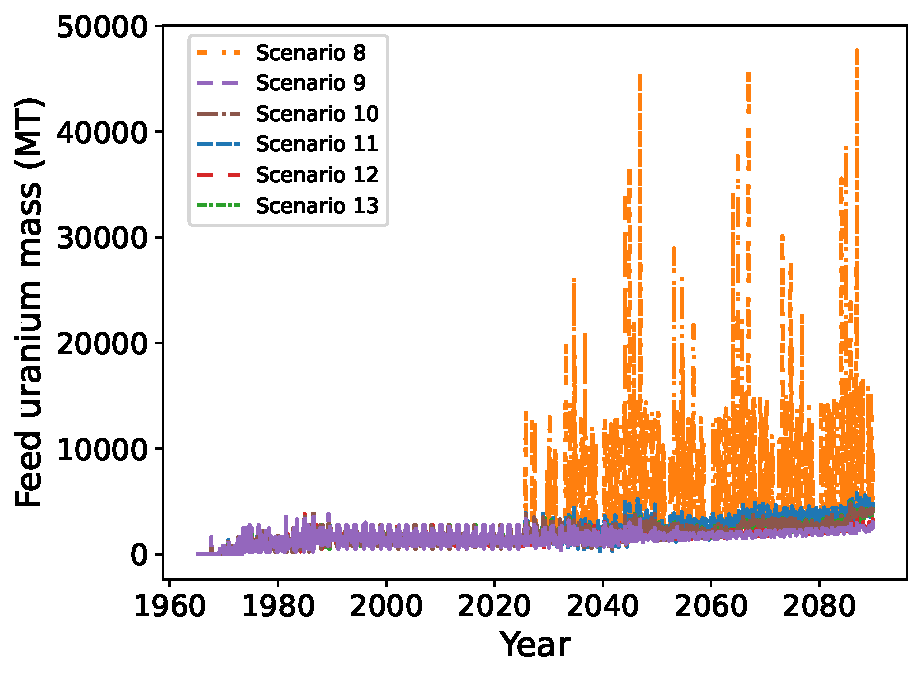
\includegraphics[width=\textwidth]{1percent_feed.pdf}
        \caption{Mass of feed uranium to produce enriched uranium sent to 
        all reactors between 1965-2090.}
        \label{fig:1percent_all_feed}
    \end{subfigure}
    \hfill
    \begin{subfigure}[b]{0.45\textwidth}
        \centering
        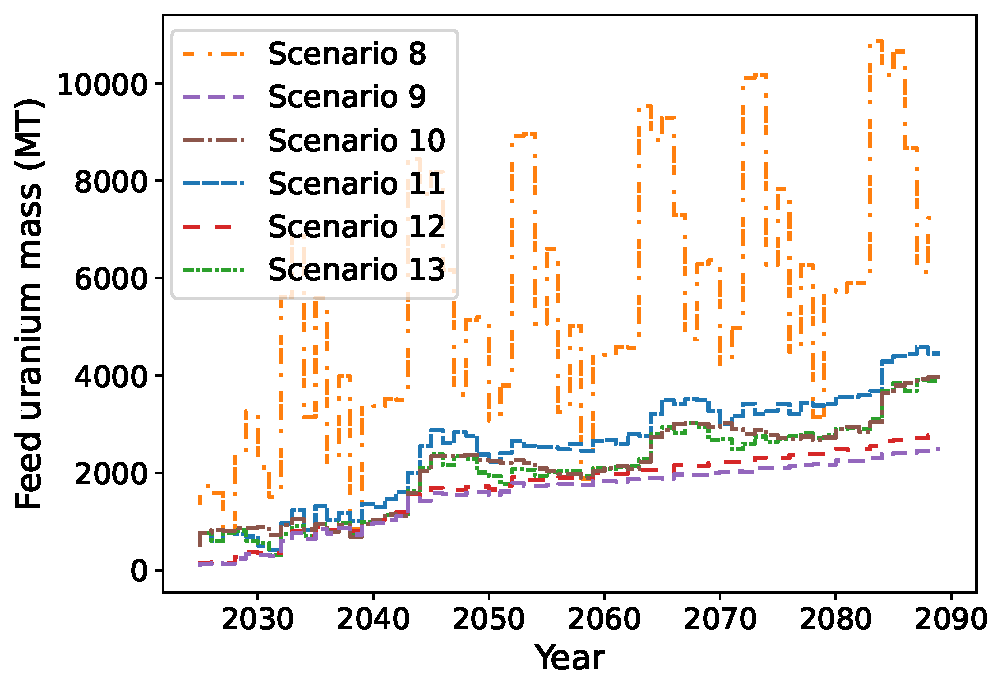
\includegraphics[width=\textwidth]{1percent_AR_feed.pdf}
        \caption{Mass of feed uranium to produce enriched uranium sent to 
        advanced reactors between 2025-2090.}
        \label{fig:1percent_AR_feed}
    \end{subfigure}
    \begin{subfigure}[b]{0.45\textwidth}
        \centering
        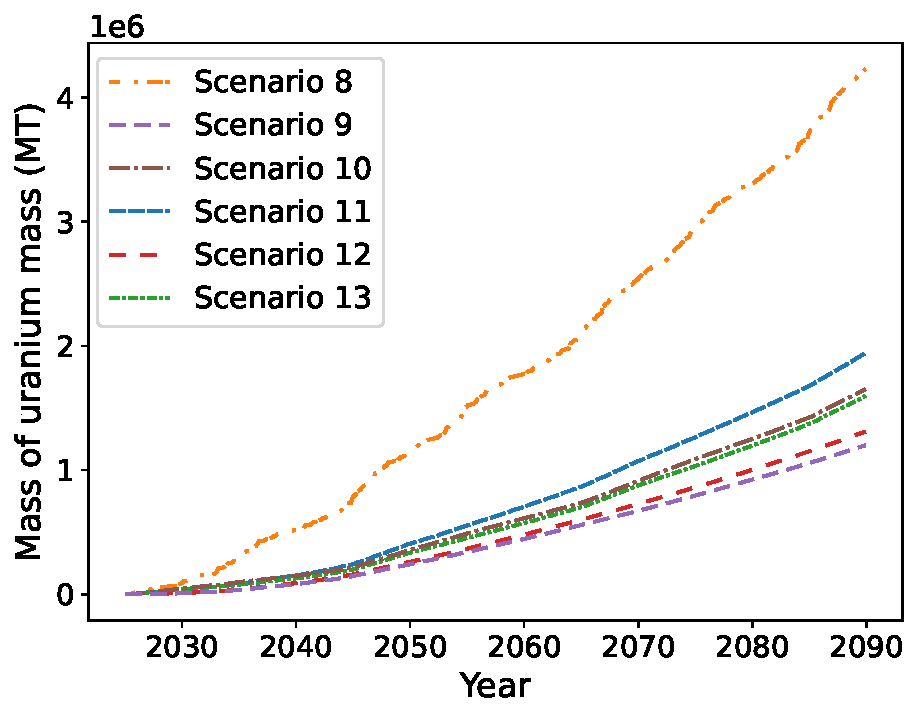
\includegraphics[width=\textwidth]{1percent_feed_cumulative.pdf}
        \caption{Cumulative mass of feed uranium to produce enriched uranium sent to 
        advanced reactors between 2025-2090.}
        \label{fig:1percent_feed_cumulative}
    \end{subfigure}
       \caption{Total mass of feed uranium required to produce enriched uranium
       at each time step in Scenarios 8-13.}
       \label{fig:1percent_feed}
\end{figure}

\begin{table}
    \centering 
    \caption{Metrics for feed uranium required by advanced reactors 
    between 2025-2090 in Scenarios 8-13.}
    \label{tab:1percent_feed}
    \begin{tabular}{c c c c c}
        \hline
        Scenario & Average (t/month) & \gls{HALEU} Average  
        (t/month) & Maximum (t) & Cumulative (t)\\\hline
        8 & 2,653 & 2,653 & 19,741 & 2,066,696\\
        9 & 1,706 & 1,706 & 3,547 & 1,329,338\\
        10 & 1,809 & 1,809 & 4,500 & 1,409617\\
        11 & 2,008 & 103.8 & 7,751 & 1,564,804\\
        12 & 1,777 & 1,295 & 3,626 & 1,384,507\\
        13 & 1,840 & 1,508 & 4,379 & 1,433,674\\
        \hline
    \end{tabular}
\end{table}

\section{SWU capacity}
\subsection{No growth scenarios}
The \gls{SWU} capacity required to produce the enriched uranium for 
the no growth scenarios follows a similar pattern as 
the feed uranium required by each scenario (Figure \ref{fig:nogrowth_swu}, 
Table \ref{tab:nogrowth_swu}). Scenario 2 requires the largest monthly 
average capacity, average capacity to produce \gls{HALEU}, and maximum 
capacity needed. Scenario 3 requires the smallest average for the total 
\gls{SWU} capacity and Scenario 6 requires the smallest average 
\gls{SWU} capacity to produce \gls{HALEU}. Scenario 3 requires the least 
\gls{SWU} capacity because it deploys only Xe-100s, which require the 
smallest \gls{SWU} capacity to produce a core-load of fuel. 
Scenario 6 requires the smallest \gls{SWU} capacity to produce \gls{HALEU}
because most of the enriched uranium is for the 
VOYGRs. Scenarios 2, 5, and 7 require a larger average \gls{SWU} capacity 
than the \glspl{LWR} before 2025. 

\begin{figure}
    \centering
    \begin{subfigure}[b]{0.45\textwidth}
        \centering
        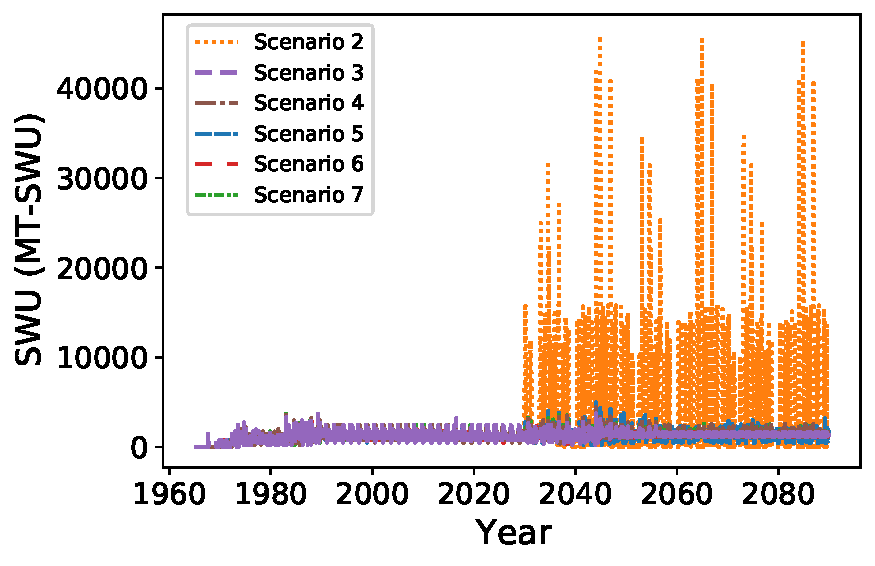
\includegraphics[width=\textwidth]{nogrowth_SWU.pdf}
        \caption{\gls{SWU} capacity required to enrich the mass of 
        uranium sent to all reactors between 1965-2090.}
        \label{fig:nogrowth_all_SWU}
    \end{subfigure}
    \hfill
    \begin{subfigure}[b]{0.45\textwidth}
        \centering
        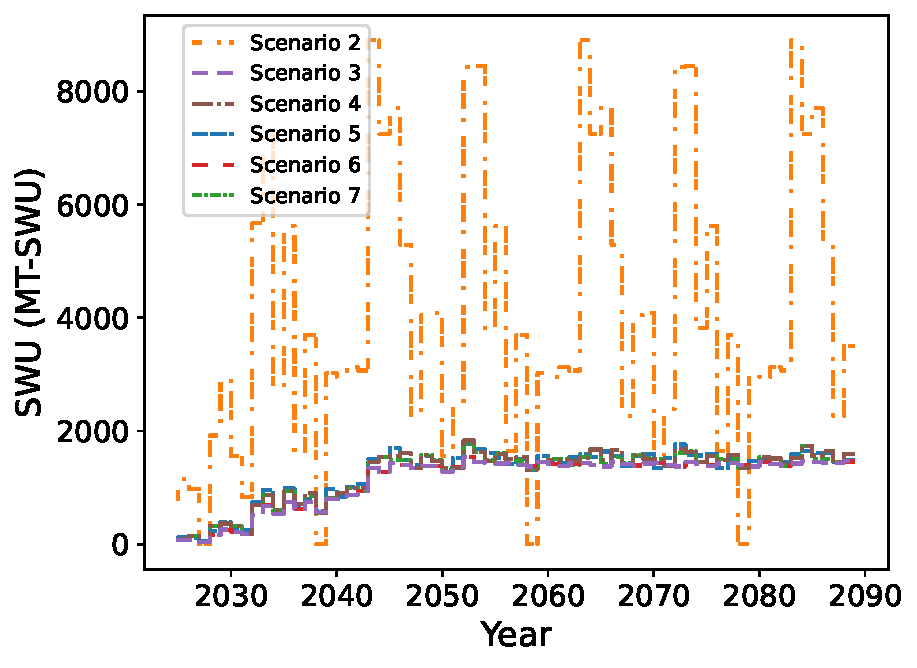
\includegraphics[width=\textwidth]{nogrowth_AR_SWU.pdf}
        \caption{\gls{SWU} capacity required to enrich the mass of 
        uranium sent to advanced reactors between 2025-2090.}
        \label{fig:nogrowth_AR_SWU}
    \end{subfigure}
       \caption{\gls{SWU} capacity required to produce enriched uranium 
       for reactors in Scenarios 2-7.}
       \label{fig:nogrowth_swu}
\end{figure}

\begin{table}
    \centering 
    \caption{Metrics for \gls{SWU} capacity to enrich uranium for 
    advanced reactors between 2025-2090 in Scenarios 2-7.}
    \label{tab:nogrowth_swu}
    \begin{tabular}{c c c c}
        \hline
        Scenario & Average  (t-SWU/month) & Average
        for \gls{HALEU} (t-SWU/month) & Maximum (t-SWU)\\\hline
        2 & 3,993 & 3,993 & 45,424 \\
        3 & 1,086 & 1,086 & 2,991\\
        4 & 1,161 & 1,161 & 3,683\\
        5 & 2,674 & 2,210 & 41,548 \\
        6 & 1,095 & 318.3 & 4,678\\
        7 & 1,522 & 1,244 & 26,459\\
        \hline
    \end{tabular}
\end{table}

The \gls{SWU} capacity required to produce \gls{HALEU} decreases when 
deploying the VOYGR along with the other reactors, with the exception 
of deploying the VOYGR with both \gls{HALEU}-fueled reactors, as noted 
with the feed uranium requirements. 
Scenario 6 requires the least \gls{SWU} capacity to produce 
\gls{HALEU}, despite requiring the largest average mass of enriched 
uranium. This result arises because most of the enriched uranium in this 
scenario is for VOYGRs, which don't require \gls{HALEU}. This 
scenario demonstrates how a decrease in the product assay decreases 
the \gls{SWU} requirements despite an increase in the product mass. 

The maximum \gls{SWU} capacity required to meet enriched uranium demand 
varies between 2.7-15.5 times the monthly average for all \gls{SWU}. 
The magnitude differences between the average and the maximum pose potential 
problems for facility design and nonproliferation safeguards. Facilities 
will likely need to be built at a capacity greater than the average 
monthly requirement in order to produce enough enriched uranium to meet 
the peak demands. However, such a design may result in idle enrichment 
capacity during time periods in which the additional capacity is 
not needed to meet peaks, which poses a proliferation risk. 

\subsection{1\% growth scenarios}
The \gls{SWU} capacity required to meet the enriched uranium demand of 
the 1\% growth scenarios 
follows the same patterns as the \gls{SWU} capacity required in the no 
growth scenarios (Figure \ref{fig:1percent_swu}, Table \ref{tab:1percent_swu}).
Scenario 8 requires the largest average \gls{SWU} 
capacity and the largest \gls{SWU} capacity to create \gls{HALEU}. 
Scenario 11 requires the smallest average \gls{SWU} capacity for all 
advanced reactors and \gls{SWU} capacity to create \gls{HALEU}. Comparing 
the average capacity and the average capacity to produce \gls{HALEU} 
shows that most or all of the \gls{SWU} capacity needed is to produce 
\gls{HALEU}, except in Scenario 11. The 
maximum \gls{SWU} capacity required ranges between 2.1-7.4 times 
the average \gls{SWU} capacity required by each scenario. 

\begin{figure}
    \centering
    \begin{subfigure}[b]{0.45\textwidth}
        \centering
        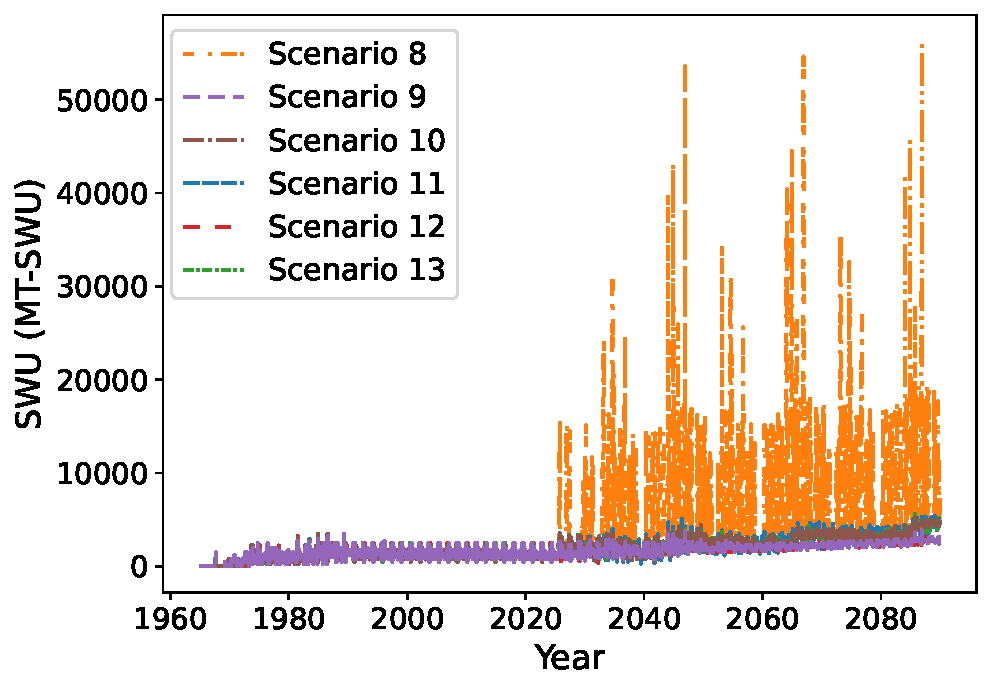
\includegraphics[width=\textwidth]{1percent_SWU.pdf}
        \caption{\gls{SWU} capacity required to enrich the mass of 
        uranium sent to all reactors between 1965-2090.}
        \label{fig:1percent_all_SWU}
    \end{subfigure}
    \hfill
    \begin{subfigure}[b]{0.45\textwidth}
        \centering
        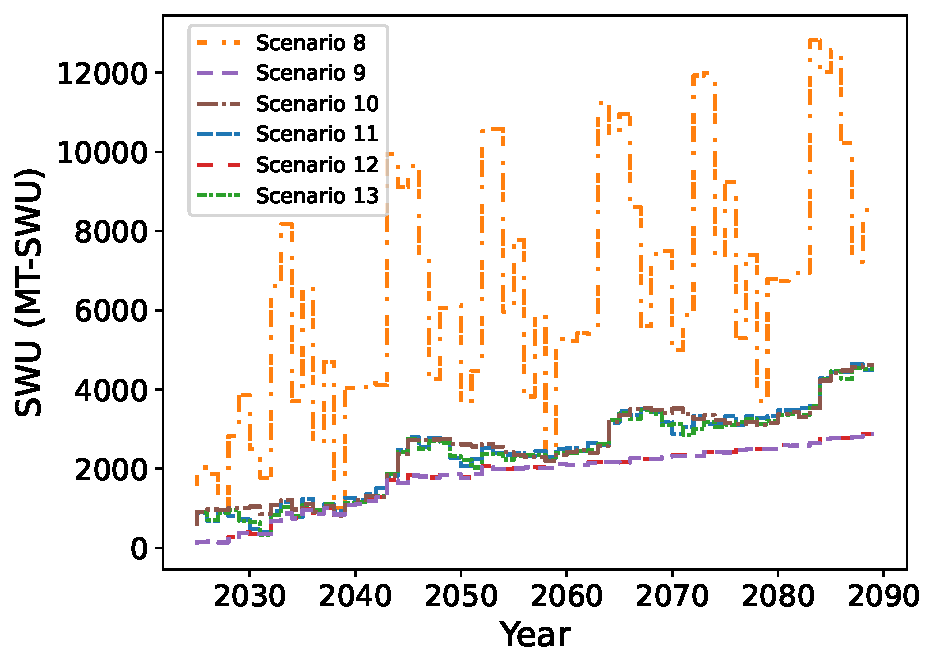
\includegraphics[width=\textwidth]{1percent_AR_SWU.pdf}
        \caption{\gls{SWU} capacity required to enrich the mass of 
        uranium sent to advanced reactorsbetween 2025-2090.}
        \label{fig:1percent_AR_SWU}
    \end{subfigure}
       \caption{\gls{SWU} capacity required to produce enriched uranium 
       for reactors in Scenarios 8-13.}
       \label{fig:1percent_swu}
\end{figure}

\begin{table}
    \centering 
    \caption{Metrics for \gls{SWU} capacity to enrich uranium for 
    advanced reactors between 2025-2090 in Scenarios 8-13.}
    \label{tab:1percent_swu}
    \begin{tabular}{c c c c}
        \hline
        Scenario & Average (t-SWU/month) & Average  
        for \gls{HALEU} (t-SWU/month) & Maximum (t-SWU)\\\hline
        8 & 2,993 & 2,993 & 22,268 \\
        9 & 1,964 & 1,964 & 4,083 \\
        10 & 2,076 & 2,076 & 5,149\\
        11 & 1,806 & 117.0 & 6,872 \\
        12 & 1,919 & 1,491 & 4,059\\
        13 & 2,025 & 1,730 & 4,469\\
        \hline
    \end{tabular}
\end{table}

\section{Waste}
The final metric of interest for the once-through transition scenarios is 
the amount of \gls{SNF} waste that must be disposed of, referred to as waste 
for the purposes of this work. 
The amount of waste produced in a \gls{NFC} has implications on the options 
to treat and store the waste. A once-through fuel cycle will dispose of 
all of the 
waste discharged from the reactors, although 
the timing is affected by the duration in wet storage. The waste masses 
reported here are the masses discharged from the reactors, which 
matches the capacity needs for disposal in a dry storage system or a 
geologic repository, but not necessarily the timing of the disposal. The 
disposal of \gls{HALEU} and non-\gls{HALEU} fuel will likely take similar 
forms, so there is no separation between the two in this work. The masses 
presented here are the masses of all materials in the \gls{SNF}, not just 
the uranium discharged, because all materials in the \gls{SNF} must be 
disposed of, not just the uranium. 

\subsection{No growth scenarios}
The magnitude of discharged from the advanced reactors 
(Figure \ref{fig:nogrowth_waste}) follows the same pattern as the enriched 
uranium masses, but with delayed timing. This pattern matches expectations, 
because all of the material that enters each reactor is discharged in this 
\gls{NFC}. The values of the masses discharged are different than those 
of the enriched uranium masses for two reasons. The first is that the 
\gls{SNF} masses include any carbon or oxygen in the fuel forms, which 
are not included in the enriched uranium masses. The second is because the 
fuel in the reactors at the simulation are not included in these 
calculations, because they are not traded to the cooling pool facility.
Scenario 6 experiences the largest average mass of \gls{SNF} 
discharged but the smallest average mass of \gls{HALEU} discharged,
which is consistent with the mass of enriched uranium.
The average mass of \gls{SNF} discharged by advanced reactors is less than 
the average discharged in Scenario 1. This result 
suggests \gls{HALEU}-fueled reactors may decrease the amount of \gls{SNF}
to disposed of in a once-through fuel cycle. 


\begin{figure}
    \centering
    \begin{subfigure}[b]{0.45\textwidth}
        \centering
        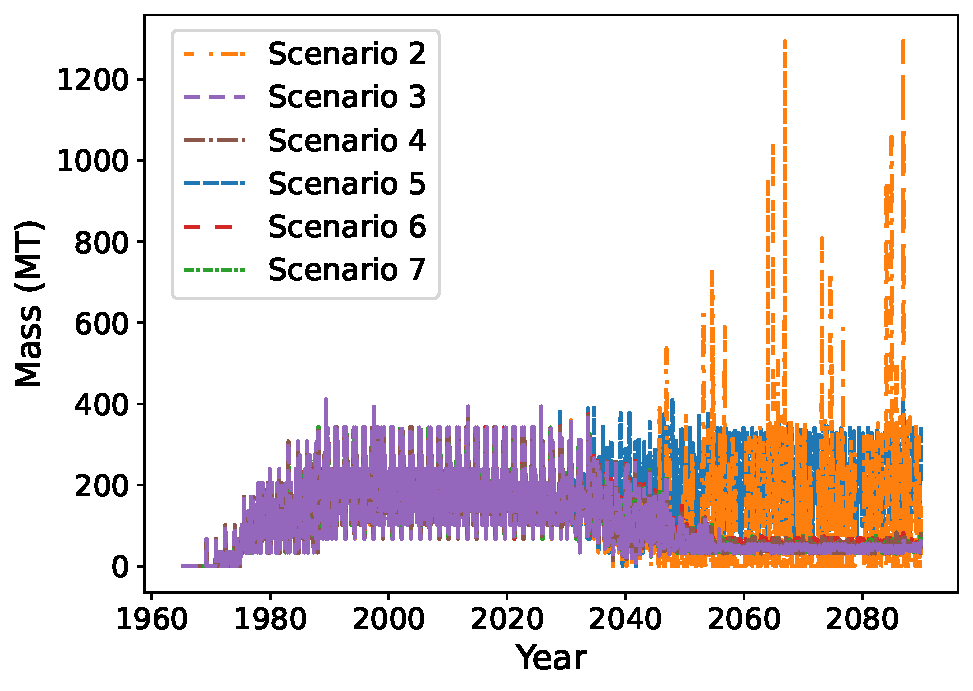
\includegraphics[width=\textwidth]{nogrowth_waste.pdf}
        \caption{Mass of fuel discharged from all reactors 
        between 1965-2090.}
        \label{fig:nogrowth_all_waste}
    \end{subfigure}
    \hfill
    \begin{subfigure}[b]{0.45\textwidth}
        \centering
        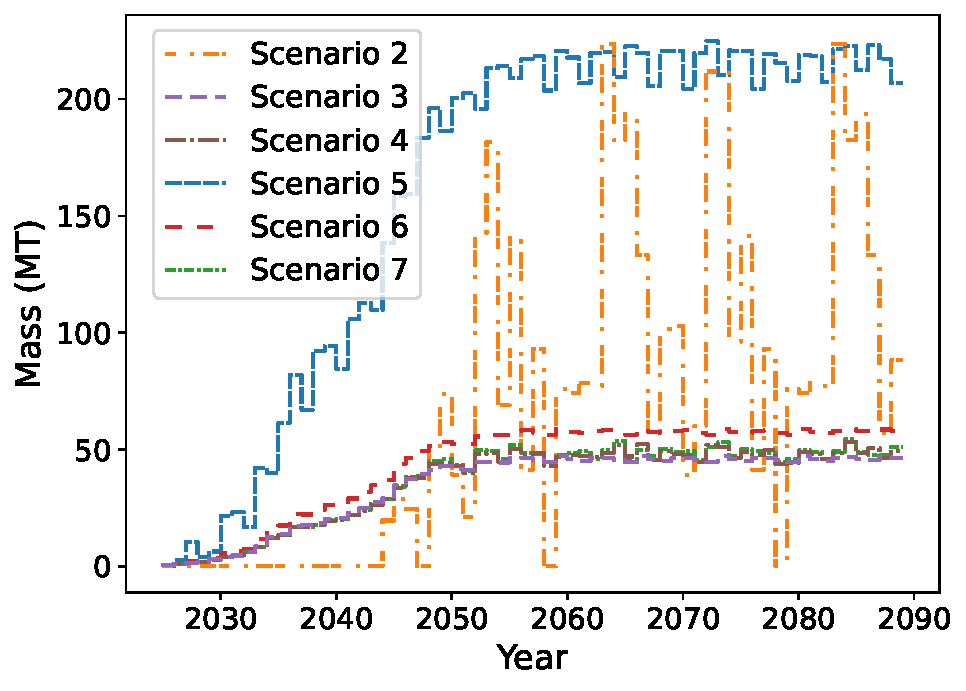
\includegraphics[width=\textwidth]{nogrowth_AR_waste.pdf}
        \caption{Mass of fuel discharged from advanced reactors 
        between 2025-2090.}
        \label{fig:nogrowth_AR_waste}
    \end{subfigure}
    \begin{subfigure}[b]{0.45\textwidth}
        \centering
        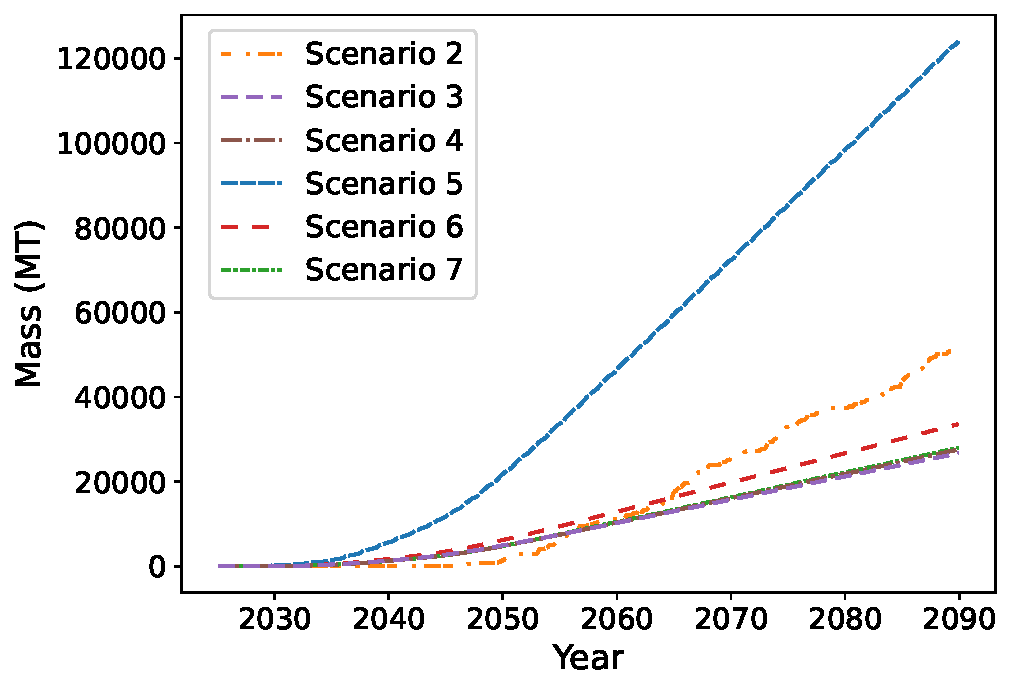
\includegraphics[width=\textwidth]{nogrowth_waste_cumulative.pdf}
        \caption{Cumulative mass of fuel discharged from advanced reactors 
        between 2025-2090.}
        \label{fig:nogrowth_waste_cumulative}
    \end{subfigure}
       \caption{Mass of fuel discharged from reactors 
       as a function of time for Scenarios 2-7. }
       \label{fig:nogrowth_waste}
\end{figure}

\begin{table}
    \centering 
    \caption{Metrics for waste discharged from advanced reactors 
    between 2025-2090 in Scenarios 2-7.}
    \label{tab:nogrowth_waste}
    \begin{tabular}{c c c c c}
        \hline
        Scenario & Average (t/month) & Average of \gls{HALEU} 
        (t/month) & Maximum (t) & Cumulative (t)\\\hline
        2 & 66.15 & 66.15 & 1,142 & 51,531\\
        3 & 32.81 & 32.81 & 55.29 & 25,560\\
        4 & 33.65 & 33.65 & 76.75 & 26,210\\
        5 & 107.7 & 43.99 & 1,108 & 83,925\\
        6 & 124.9 & 9.607 & 331.2 & 97,302\\
        7 & 73.05 & 31.78 & 748.2 & 56,905\\
        \hline
    \end{tabular}
\end{table}

The first \gls{SNF} discharged from advanced reactors is in August 
2030 for Scenarios 3, 4, and 6, April 2031 in Scenario 7, February 2032 
in Scenario 5, and 
February 2050 in Scenario 2. The differences in timing of first \gls{SNF} 
discharge from advanced reactors is a result of the refueling scheme of 
each type of reactor. Xe-100s, deployed in Scenarios 3, 4, 6, 
and 7, utilize online refueling and discharge \gls{SNF} 
every 6 months, results in the first discharge soon after their initial 
deployment. VOYGRs, deployed in Scenarios 4, 5, 6, and 7, have an 
18-month refueling cycle, so the first \gls{SNF} discharge for these 
reactors occurs 18 months after deployment. \glspl{MMR}, deployed in 
Scenarios 2, 4, 5, and 7, do not undergo refueling, so the first \gls{SNF} 
discharge occurs 20 years after first deployment. The shortest refuleing 
time of the reactors deployed in a scenario governs when 
first \gls{SNF} discharge in that scenario. Thus, the Xe-100 is the 
governing reactor for 
Scenarios 3, 4, 6, and 7 the VOYGR is the governing reactor for Scenarios  
5, and the \gls{MMR} is the governing reactor for Scenario 2 with regards 
to \gls{SNF} discharge times. In Scenario 7, \gls{SNF} is first discharged 
at a different time than in the other scenarios governed by the Xe-100
because of differences in the deployment scheme. In Scenario 7, VOYGRs and
\glspl{MMR} are first deployed in February 2030, and Xe-100s are first 
deployed in October 2030. Despite this difference in when the advanced 
reactor types are first deployed, the Xe-100 still governs the first \gls{SNF}
discharge date because they are deployed within 18 months of the first 
VOYGR deployment and within 19.5 years of the first \gls{MMR} 
deployment. This scenario demonstrates how even for the deployment of 
the same reactors, the deployment schedule affects the rate of \gls{SNF} 
discharge. 

The 
advanced reactors in all of the scenarios discharge 
less \gls{SNF} than the \glspl{LWR}. The cumulative mass of discharged 
\gls{SNF} for all of the no growth scenarios except Scenarios 5 and 6 
could be 
disposed of in a geologic repository cited in the US, which is required 
to have a capacity of at lest 70,000 MTHM \cite{noauthor_nuclear_1983}.


\subsection{1\% growth scenarios}
For the 1\% growth scenarios, similar patterns are observed to the 
no growth scenarios; Scenario 11 
has the largest average mass of \gls{SNF} discharged \gls{SNF} while also 
having the smallest average mass of discharged \gls{HALEU} \gls{SNF} 
(Figure \ref{fig:1percent_waste}, Table \ref{tab:1percent_waste}). There 
is more variation than the no growth scenarios in when each scenario 
first discharges \gls{SNF}: 
September 2046 in Scenario 8, March 2027 in Scenario 9, April 2027 in 
Scenario 10, October 2028 in Scenario 11, May 2027 in Scenario 12, and 
April 2027 in Scenario 13. All of these scenarios deploy reactors starting 
at the same time (September 2026), so it is unclear why there is so much 
variation in the first \gls{SNF} discharged. One would expect similar 
consistency to what was observed for the no growth scenarios. 

Based on the cumulative masses, the propopsed 70,000 MTHM capacity of 
a geologic repository in the US would only be able to store the \gls{SNF} 
discharged from advanced reactors in Scenarios 8, 9, and 10. Additional 
repositories or an expanded capacity of the repository would be required 
to dispose of the waste from Scenarios 11, 12, and 13. However, the 
cumulative waste discharged from advanced reactors is less than the 
cumulative mass discharged from the \glspl{LWR} in all scenarios except 
Scenario 11. 

\begin{figure}
    \centering
    \begin{subfigure}[b]{0.45\textwidth}
        \centering
        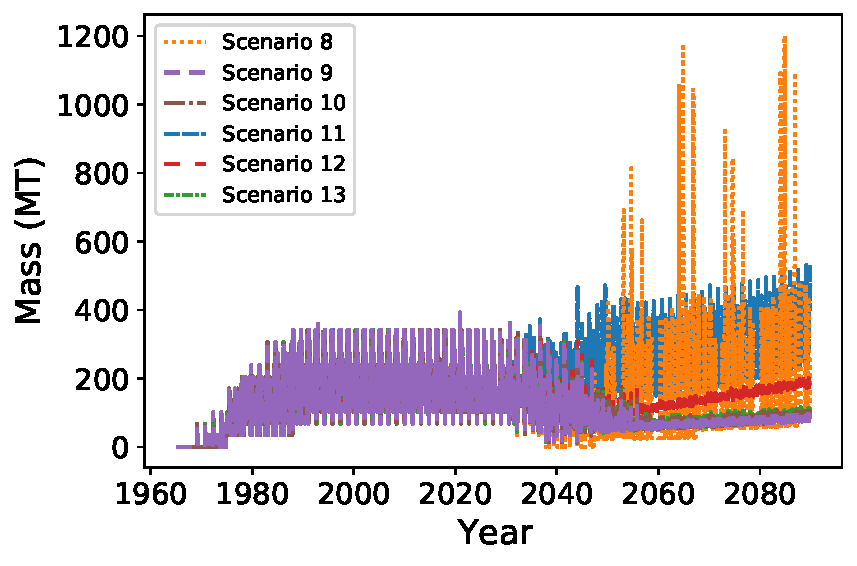
\includegraphics[width=\textwidth]{1percent_waste.pdf}
        \caption{Mass of fuel discharged from all reactors between 
        1965-2090.}
        \label{fig:1percent_all_waste}
    \end{subfigure}
    \hfill
    \begin{subfigure}[b]{0.45\textwidth}
        \centering
        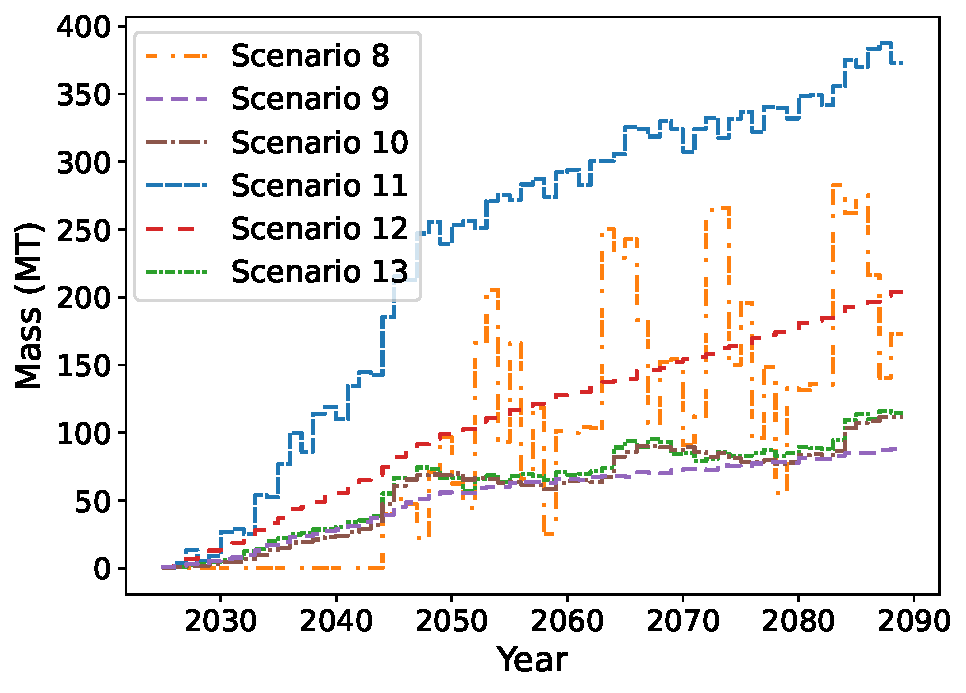
\includegraphics[width=\textwidth]{1percent_AR_waste.pdf}
        \caption{Mass of fuel discharged from advanced reactors 
        between 2025-2090.}
        \label{fig:1percent_AR_waste}
    \end{subfigure}
    \begin{subfigure}[b]{0.45\textwidth}
        \centering
        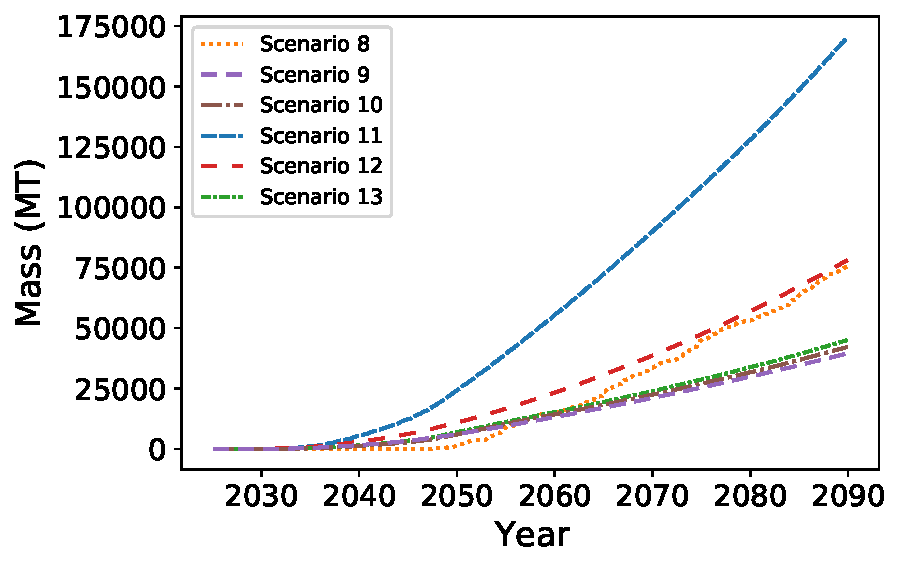
\includegraphics[width=\textwidth]{1percent_waste_cumulative.pdf}
        \caption{Cumulative mass of fuel discharged from advanced reactors 
        between 2025-2090.}
        \label{fig:1percent_waste_cumulative}
    \end{subfigure}
       \caption{Mass of fuel discharged from reactors 
       as a function of time for Scenarios 8-13. }
       \label{fig:1percent_waste}
\end{figure}

\begin{table}
    \centering 
    \caption{Metrics for waste discharged from advanced reactors 
    between 2025-2090 in Scenarios 8-13.}
    \label{tab:1percent_waste}
    \begin{tabular}{c c c c c}
        \hline
        Scenario & Average (t/month) & Average of \gls{HALEU} (t/month) 
        & Maximum (t) & Cumulative (t)\\\hline
        8 & 71.43 & 71.43 & 859.6 & 55,645 \\
        9 & 58.35 & 58.35 & 115.8 & 45,456 \\
        10 & 60.59 & 60.59 & 134.7 & 47,199 \\
        11 & 246.6 & 3.410 & 668.5 & 192,099 \\
        12 & 104.6 & 44.50 & 222.5 & 81,456 \\
        13 & 92.72 & 50.46 & 330.6 & 72,226 \\
        \hline
    \end{tabular}
\end{table}